\chapter{Analysis of Results}
\todo{Diese Seite habe ich noch nicht genau angeschaut, aber ich denke wir geben hier auch unsere grobe struktur bekannt: Satz/Testset, n-Gramm, Wörter, thought Vektor. Von Ganz aussen nach innen, sozusagen.}
In this chapter, we are going to analyze the evolution and final results of the two models (see chapter \ref{methods:both_models}), trained on the OpenSubtitles and Reddit corpus, under several different aspects. This includes the analysis of the learning process throughout the training. Then we are going to analyse the language model of the trained models and try to find a correlation between the language model in the training dataset and the language model the trained models produce.\todo{Two times model is ugly!} In the end, we are going to focus on how well the model understands and percepts them, combined with an analysis

\begin{enumerate}[noitemsep]
	\item \textbf{Quantitive}: This part focuses on evaluating metrics and other measurements. We are going to look into the metrics at train time, a similarity analysis using Sent2Vec and an analysis of the produced language models by using n-gram collocations.\todo{Not correct: What are we going to do with ngrams?}
	\item \textbf{Qualitative}: This part focuses on the quality of the language produced by the models. This includes a comparison between our models and \emph{CleverBot}\footnote{http://www.cleverbot.com/} and the development of the language model of the models throughout the training time.
	\item \textbf{Miscellaneous}: This part focuses on theoretical analysis, such as analyzing the internal embeddings for the input sequence or if and how the models are using the soft-attention mechanism in their favor.
\end{enumerate}

The analysis is done in the order listed above, that means we start by analysing the quantitive measures
\blindtext

* Attention
* Learning process
* Generated outputs over time
* Generation at the end and comparison with cleverbot and paper
* Generated outputs at the end and related ngram analysis
* Generated embeddings for input sentences
* Sent2Vec analysis

\section{How Did The Training Go?}\todo{vielleicht müssen wir den anpassen wegen neuer struktur}
First, let us start by analysing the evolution of the models with regard to the available performance metrics throughout the time span of the training. Below, in Figures~\ref{results:learning_process:metrics:opensubtitles} and~\ref{results:learning_process:metrics:reddit}, one can see the development of the loss and perplexity on the training sets for the two different models.

\paragraph{OpenSubtitles} What is eye-catching when comparing the two is that the OpenSubtitles seems to have much more variance in its performance on the validation set as opposed to the Reddit model. This probably comes from the fact that the OpenSubtitles datasets are much more noisey than the one of the Reddit model, as \cite{Vinyals:2015} also already noticed. This has to do with the fact, that we do not have any information about turn taking, which means it is certainly possible that consecutive utterances may be uttered by the same person even though we treat it if it were two persons. Also, there is the problematic with the time lags between utterances as analysed in Chapter~\ref{data:opensubtitles:time_lag_analysis}. In contrast, with the Reddit dataset, we always know who uttered a comment and hence can build a dataset which ensures that the dialogs make sense from a structural perspective.

\begin{figure}[H]
	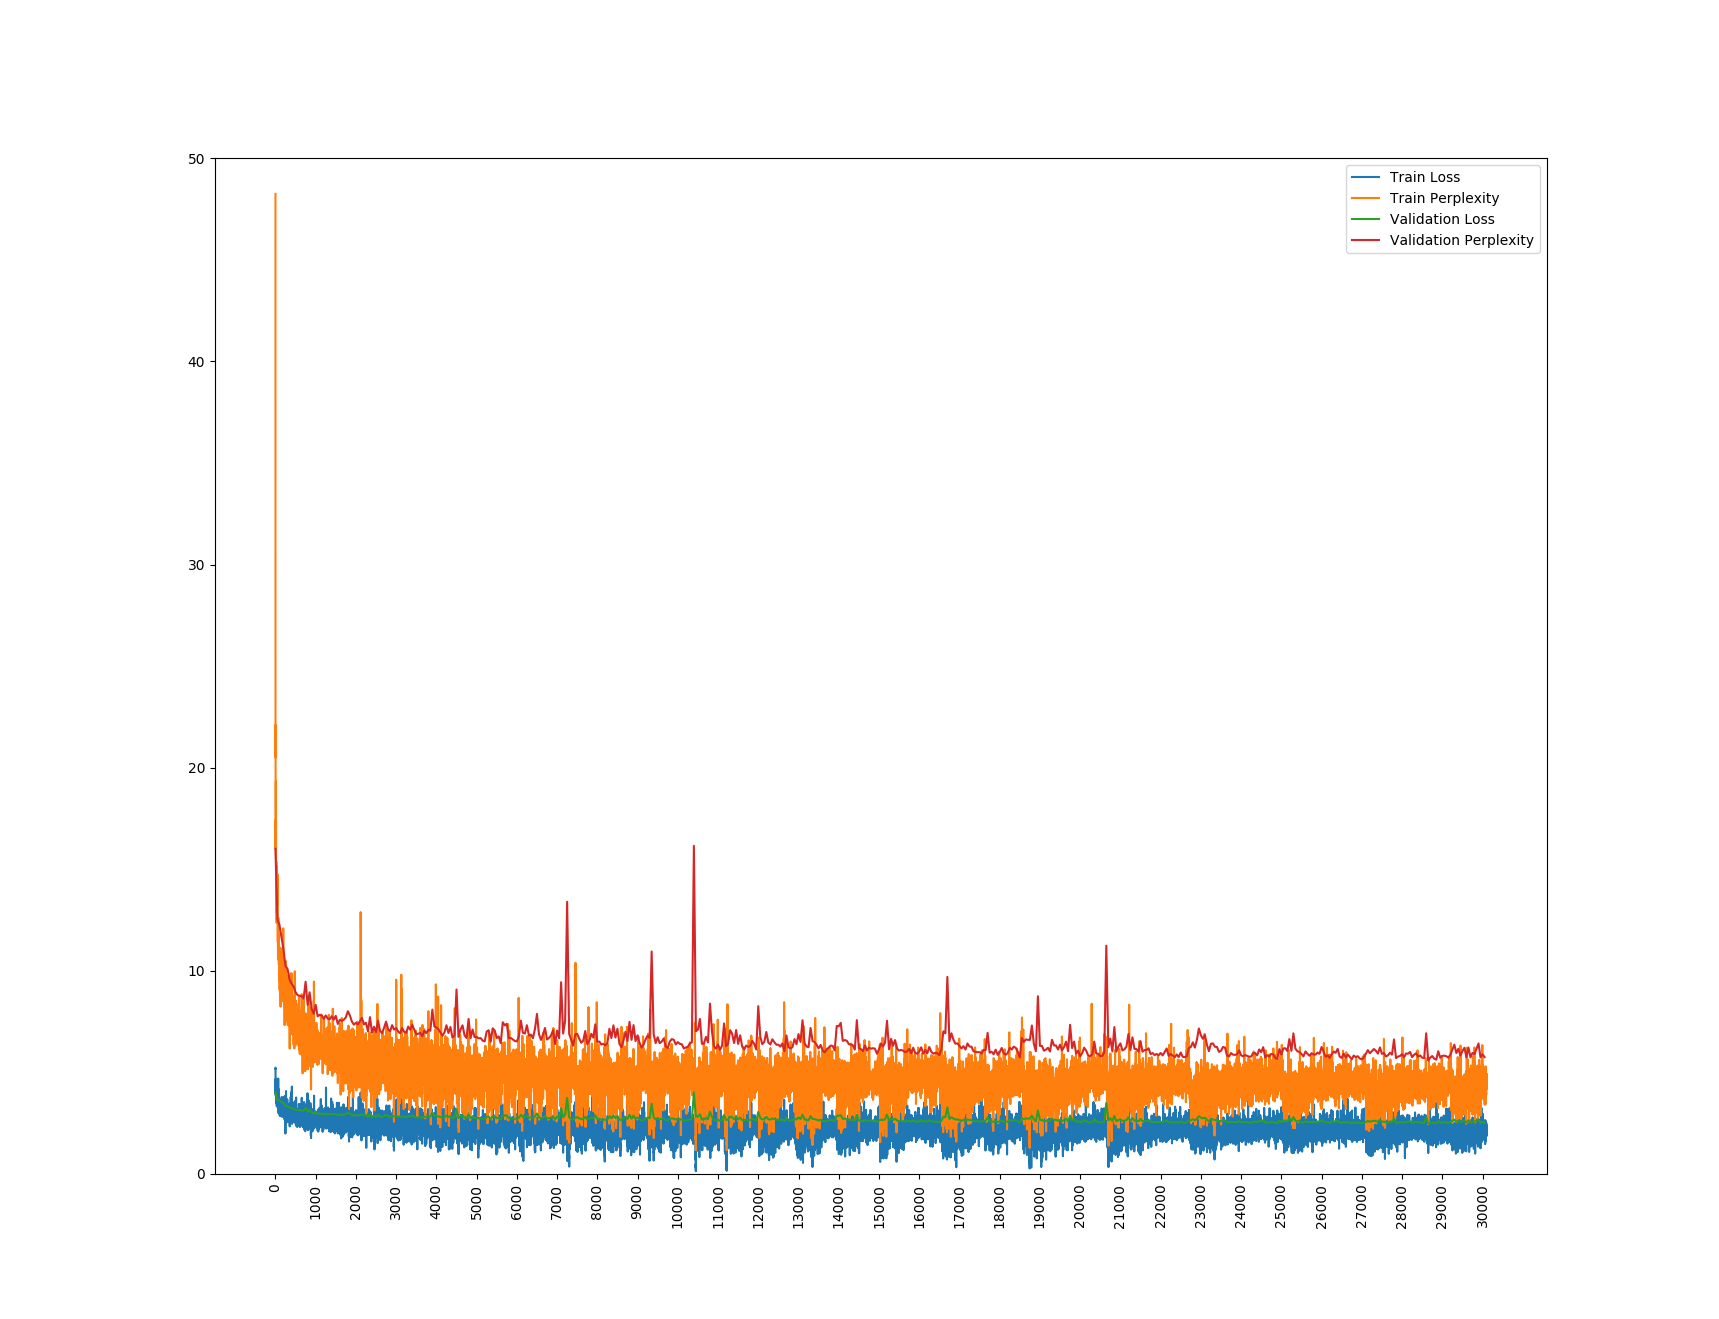
\includegraphics[width=\linewidth]{img/plots/opensubtitles_not_reversed/train_metrics.png}
	\caption{Development of the loss and perplexity on the training and validation set throughout the training of the OpenSubtitles model. One tick on the x-axis is equal to $100$ batches processed.}
	\label{results:learning_process:metrics:opensubtitles}
\end{figure}\todo{Einheiten angeben (x = 1000-er)}

\paragraph{Reddit} The learning process of the Reddit model also has a peculiarity, namely the dips in the training loss and perplexity. These dips occur about every $300'000$ to $400'000$ batches. They are also present in the development of the validation loss and perplexity, but are not as apparent as in the training metrics. We cannot explain this behaviour currently. We assume that this comes from the fact...\todo{Maybe we should be able?!} The variance however is much smaller than with the Reddit model, which strengthens our argument, that a well-structured dataset helps a lot when training such systems as it confuses the model much less.\todo{maybe rewrite this sentence somehow}

\begin{figure}[H]
	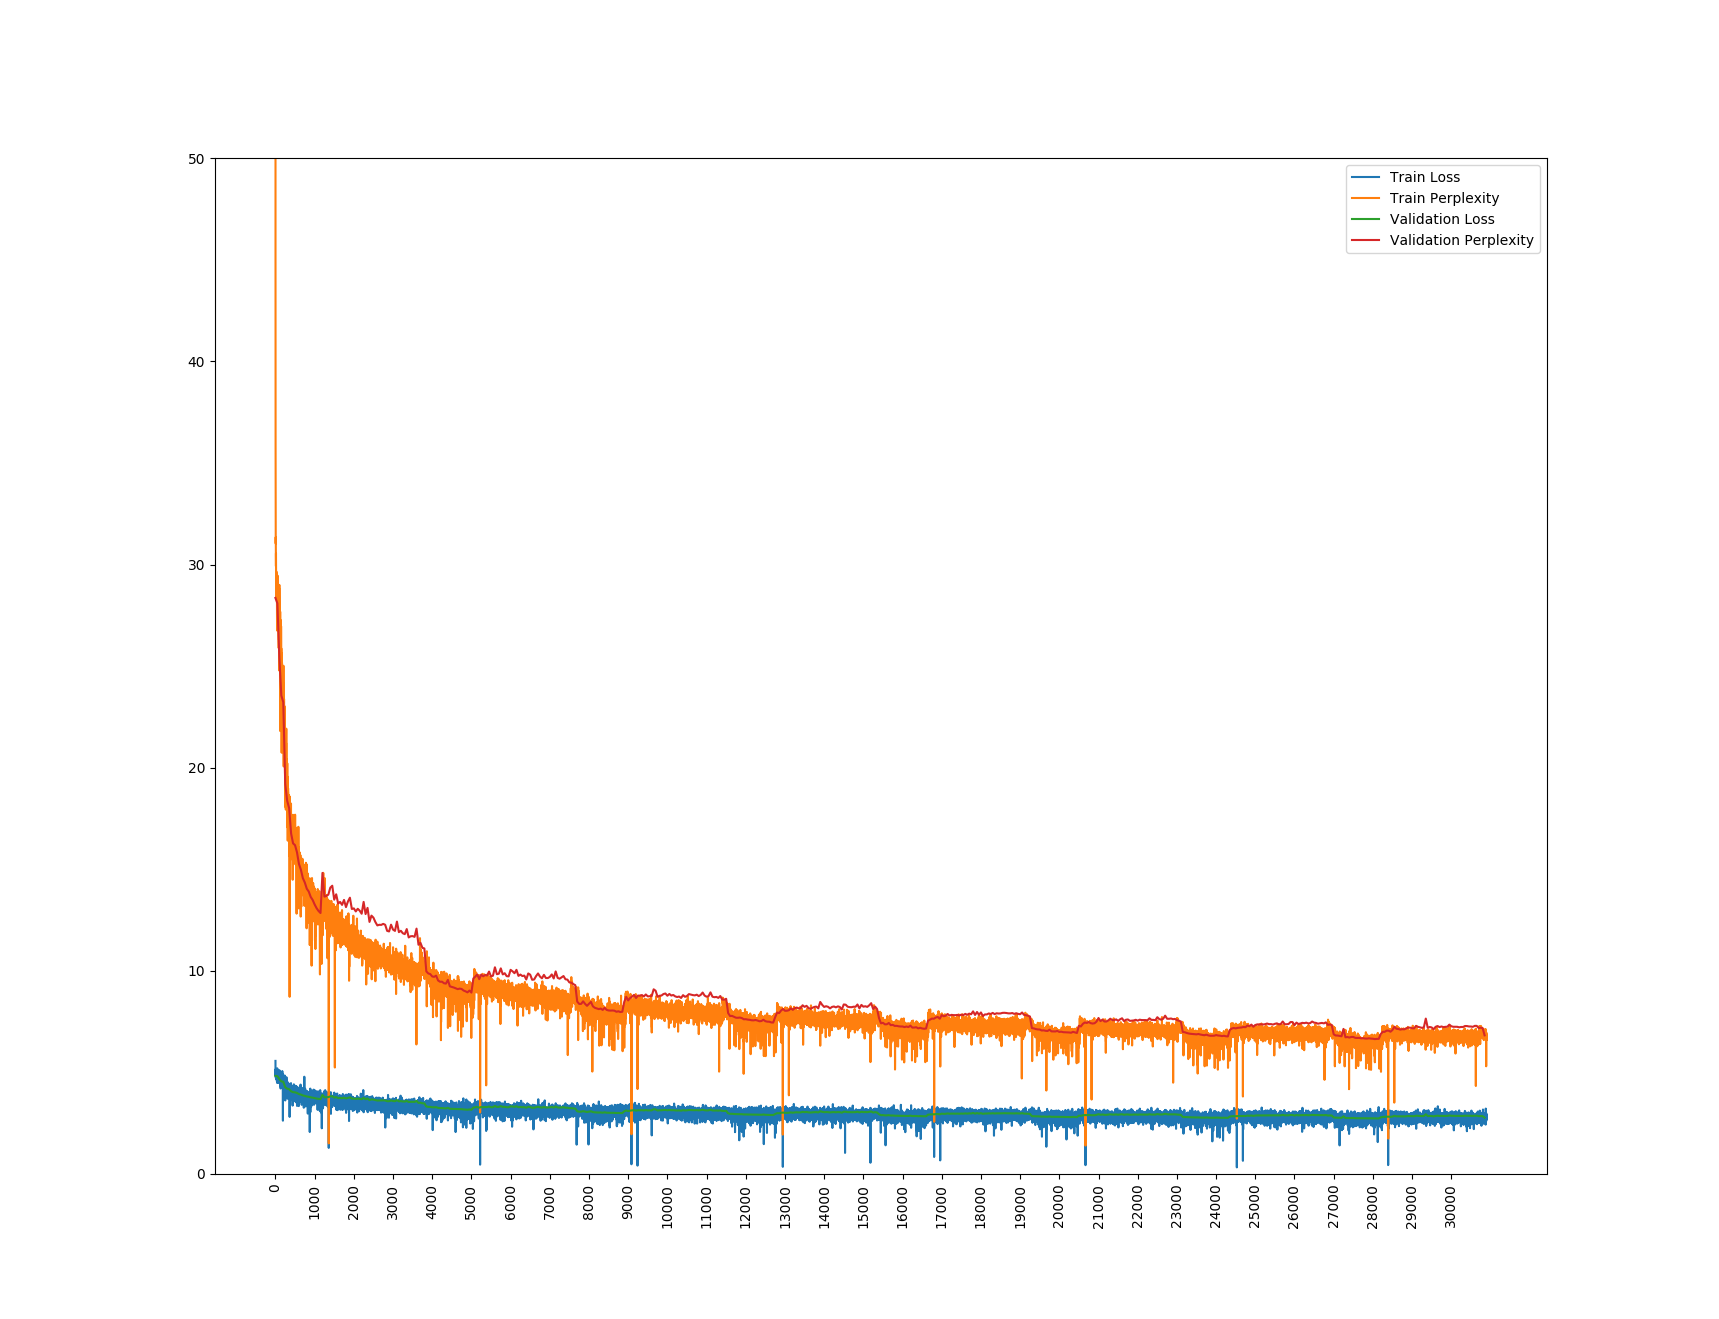
\includegraphics[width=\linewidth]{img/plots/reddit/train_metrics.png}
	\caption{Development of the loss and perplexity on the training and validation set throughout the training of the Reddit model. One tick on the x-axis is equal to $100$ batches processed.}
	\label{results:learning_process:metrics:reddit}
\end{figure}\todo{Einheiten angeben (x = 1000-er)}

\paragraph{Compared to each other}\todo{können wir auch weglassen diesen paragraphen. Weiss nicht welche Erkenntnis wir daraus ziehen können} In der Abbildung \ref{} sehen wir die loss Werte auf den Vailidierungsdaten beider Modell in einem Bild. Hier das Bild mit der valid los/perplex beider Modelle referenzieren und kurz schreiben, wer wie schnell gelernt hat und wie sich die Kurve unterscheiden. 

\paragraph{The Training Seems Successful} From the looks of the plots, it looks like the training went fine for both models, as both of them have degrading loss and perplexity. We also saw differences in how the models have evolved over the time span of the training, especially the dips in the Reddit model, but we cannot conclude anything from this right now. We are going to analyze this further and see if we can find any reasons for it. After we have analyzed the training process, we are now focusing on the performance of the models on the test datasets.

\section{Performance on Test Datasets}
After we have seen that the training process looks fine, we are going to asses the performance of these models on our test datasets. Here we use the same metrics as within the training, namely the cross-entropy loss and perplexity values. We have evaluated each model on the respective test dataset for each checkpoint we have created while training (see Chapter~\ref{methods}).

\paragraph{Surprising Results} The results on the test set are quite the opposite of the results from the training process (see Figures~\ref{result:test_performance:opensubtitles} and~\ref{result:test_performance:reddit}), where both of the models are getting worse over time. We did not expect that, but nevertheless, we are going to analyze the problem.\todo{Maybe some more clarification on what analyse means?} The results of the OpenSubtitles model seem to vary across the different checkpoints, with the best result having a perplexity of $71.07$ and a loss of $6.15$ and coming from the evaluation with the first checkpoint. The best result of the Reddit model is also achieved on the first checkpoint, with all other checkpoints having a worse perplexity. This result stands in contradiction to what we have expected. Instead of the loss going up, we would have expected it to go down in the same way as it did on the training and validation datasets. We assume, that this has to do with the cross-entropy loss and hence the perplexity being not the best fit metrics to evaluate such models, especially in a conversational context where the variety of correct answers can be immensely high. For this reason, we proposed a third performance metric, namely the usage of Sent2Vec~\cite{Pgj:2017} embeddings, to measure the similarity between the expected and generated responses. Before we are going to do this analysis, we want to take a look at different samples from both models to show that they indeed improved over time, even thought the test metrics tell a different story.

\begin{figure}[H]
	\minipage{0.5\textwidth}
	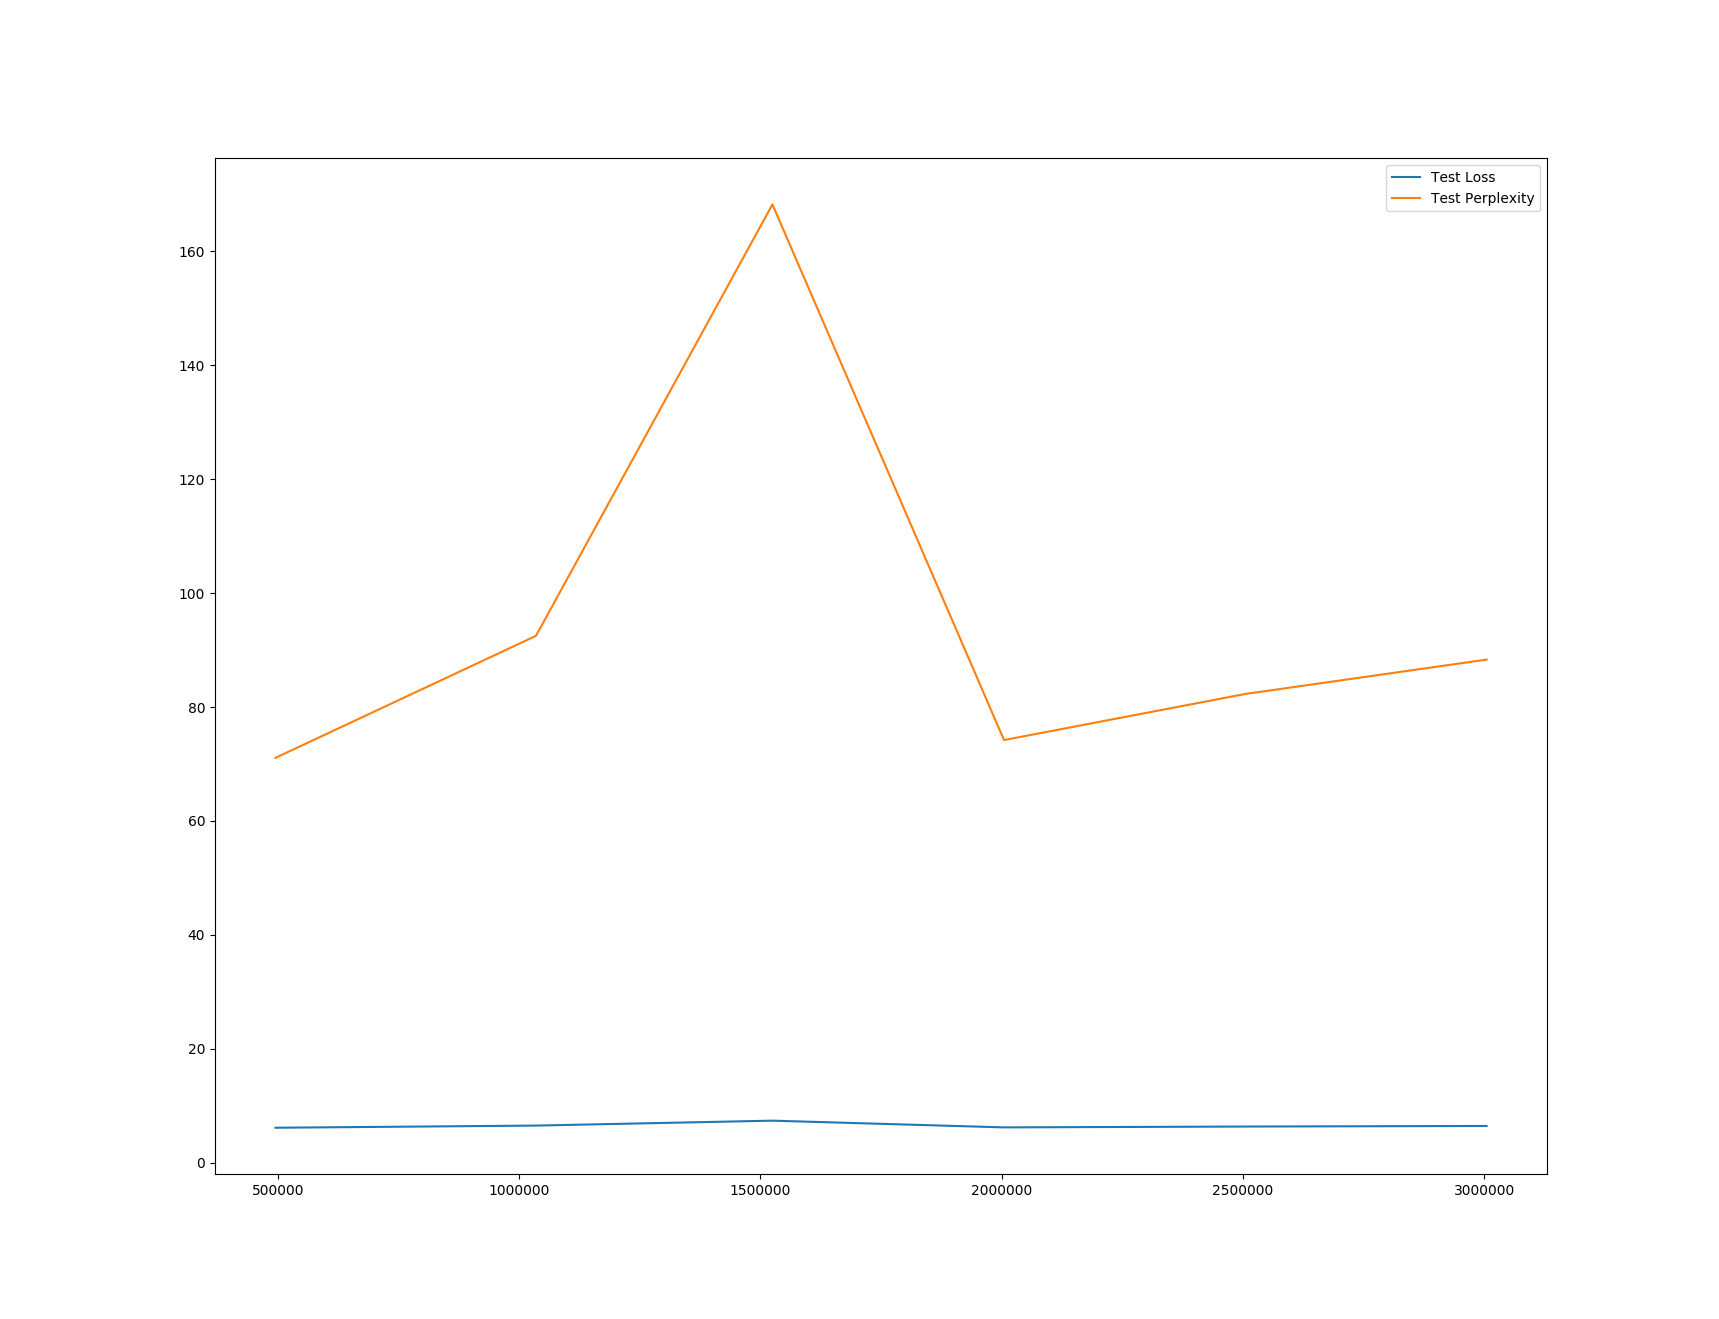
\includegraphics[width=\linewidth]{img/plots/opensubtitles_not_reversed/test_metrics_both.png}
	\centering
	\small
	\text{The loss and perplexity.}
	\endminipage\hfill
	\minipage{0.5\textwidth}
	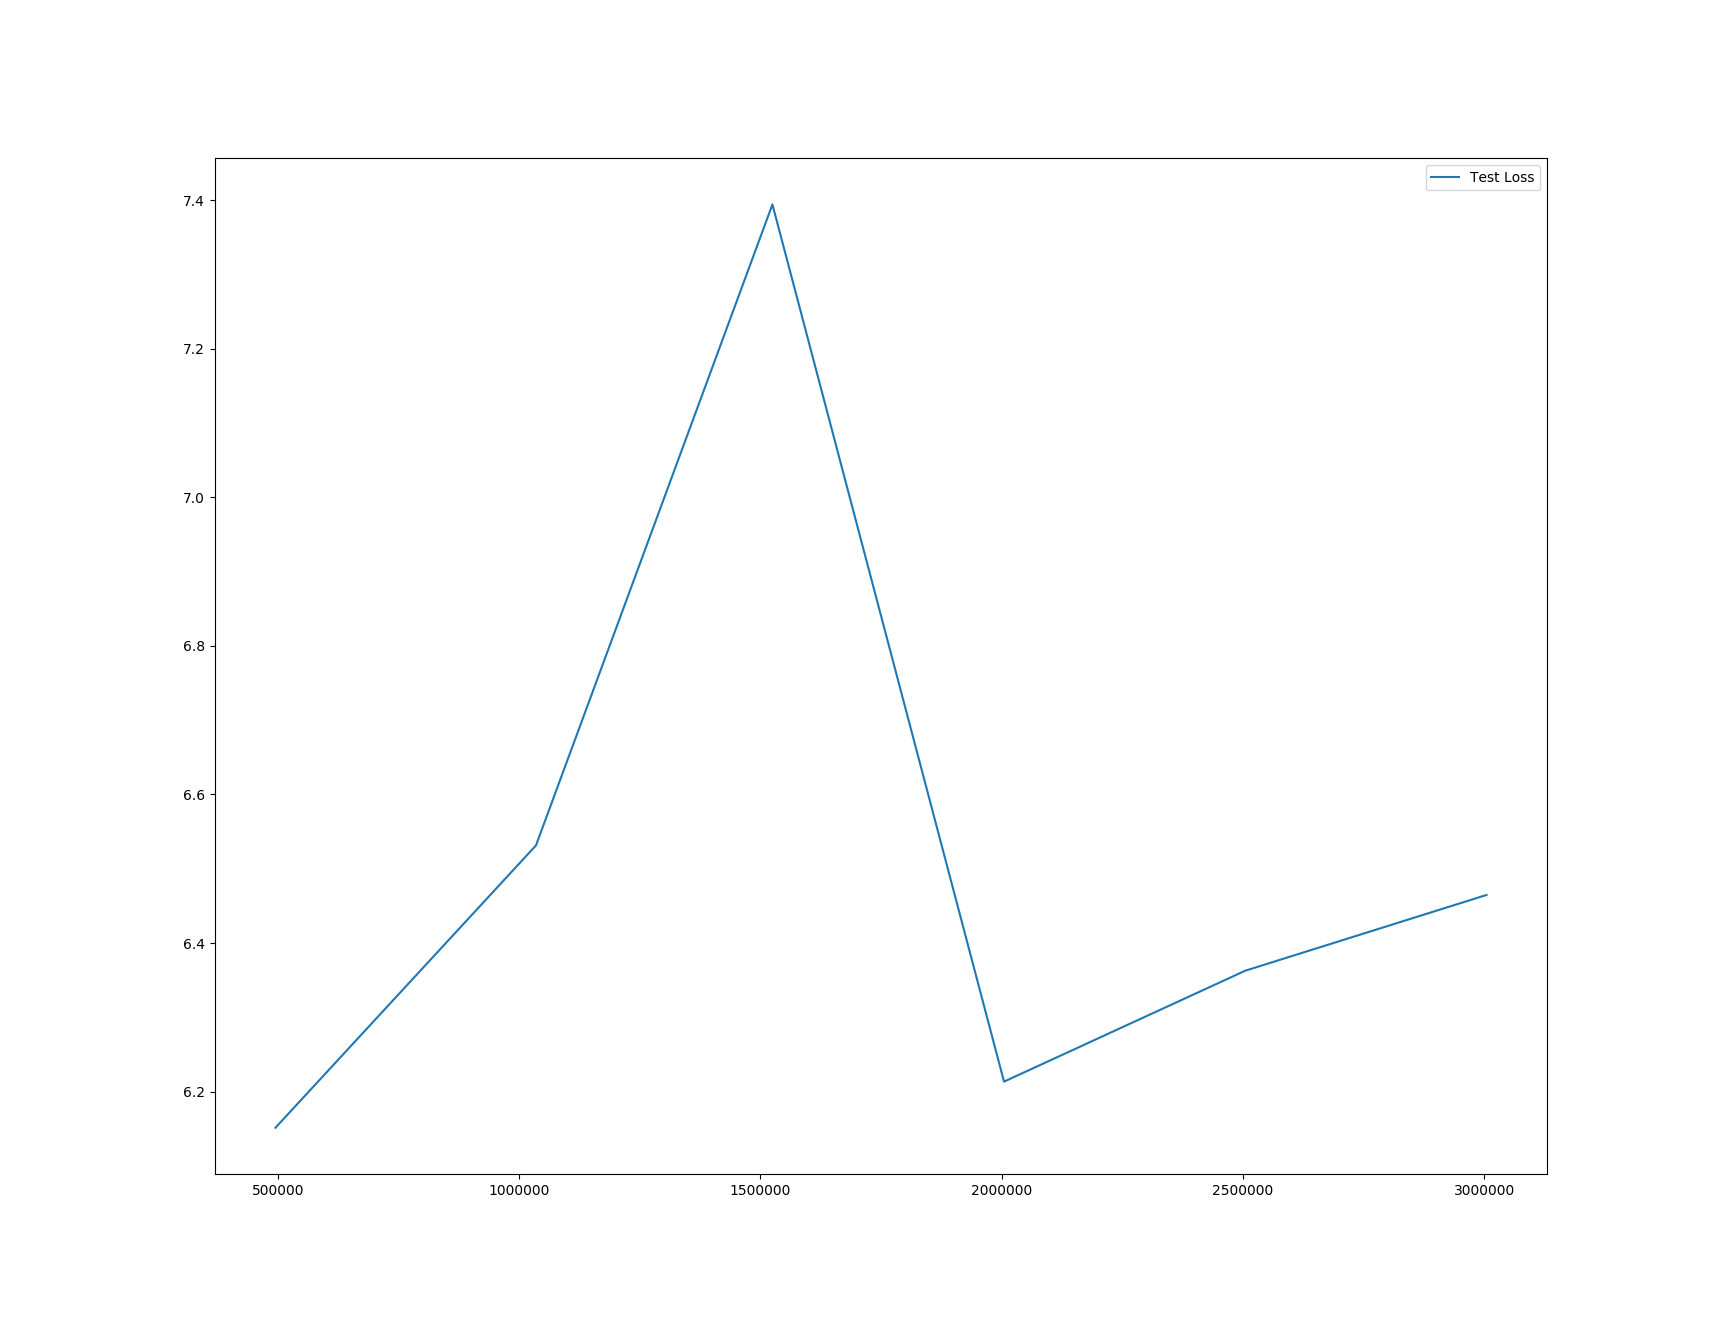
\includegraphics[width=\linewidth]{img/plots/opensubtitles_not_reversed/test_metrics_loss.png}
	\centering
	\small
	\text{Only the loss.}
	\endminipage\hfill
	\caption{The loss and perplexity by running the six different snapshots against the test dataset using the OpenSubtitles model.}
	\label{result:test_performance:opensubtitles}
\end{figure}

\begin{figure}[H]
	\minipage{0.5\textwidth}
	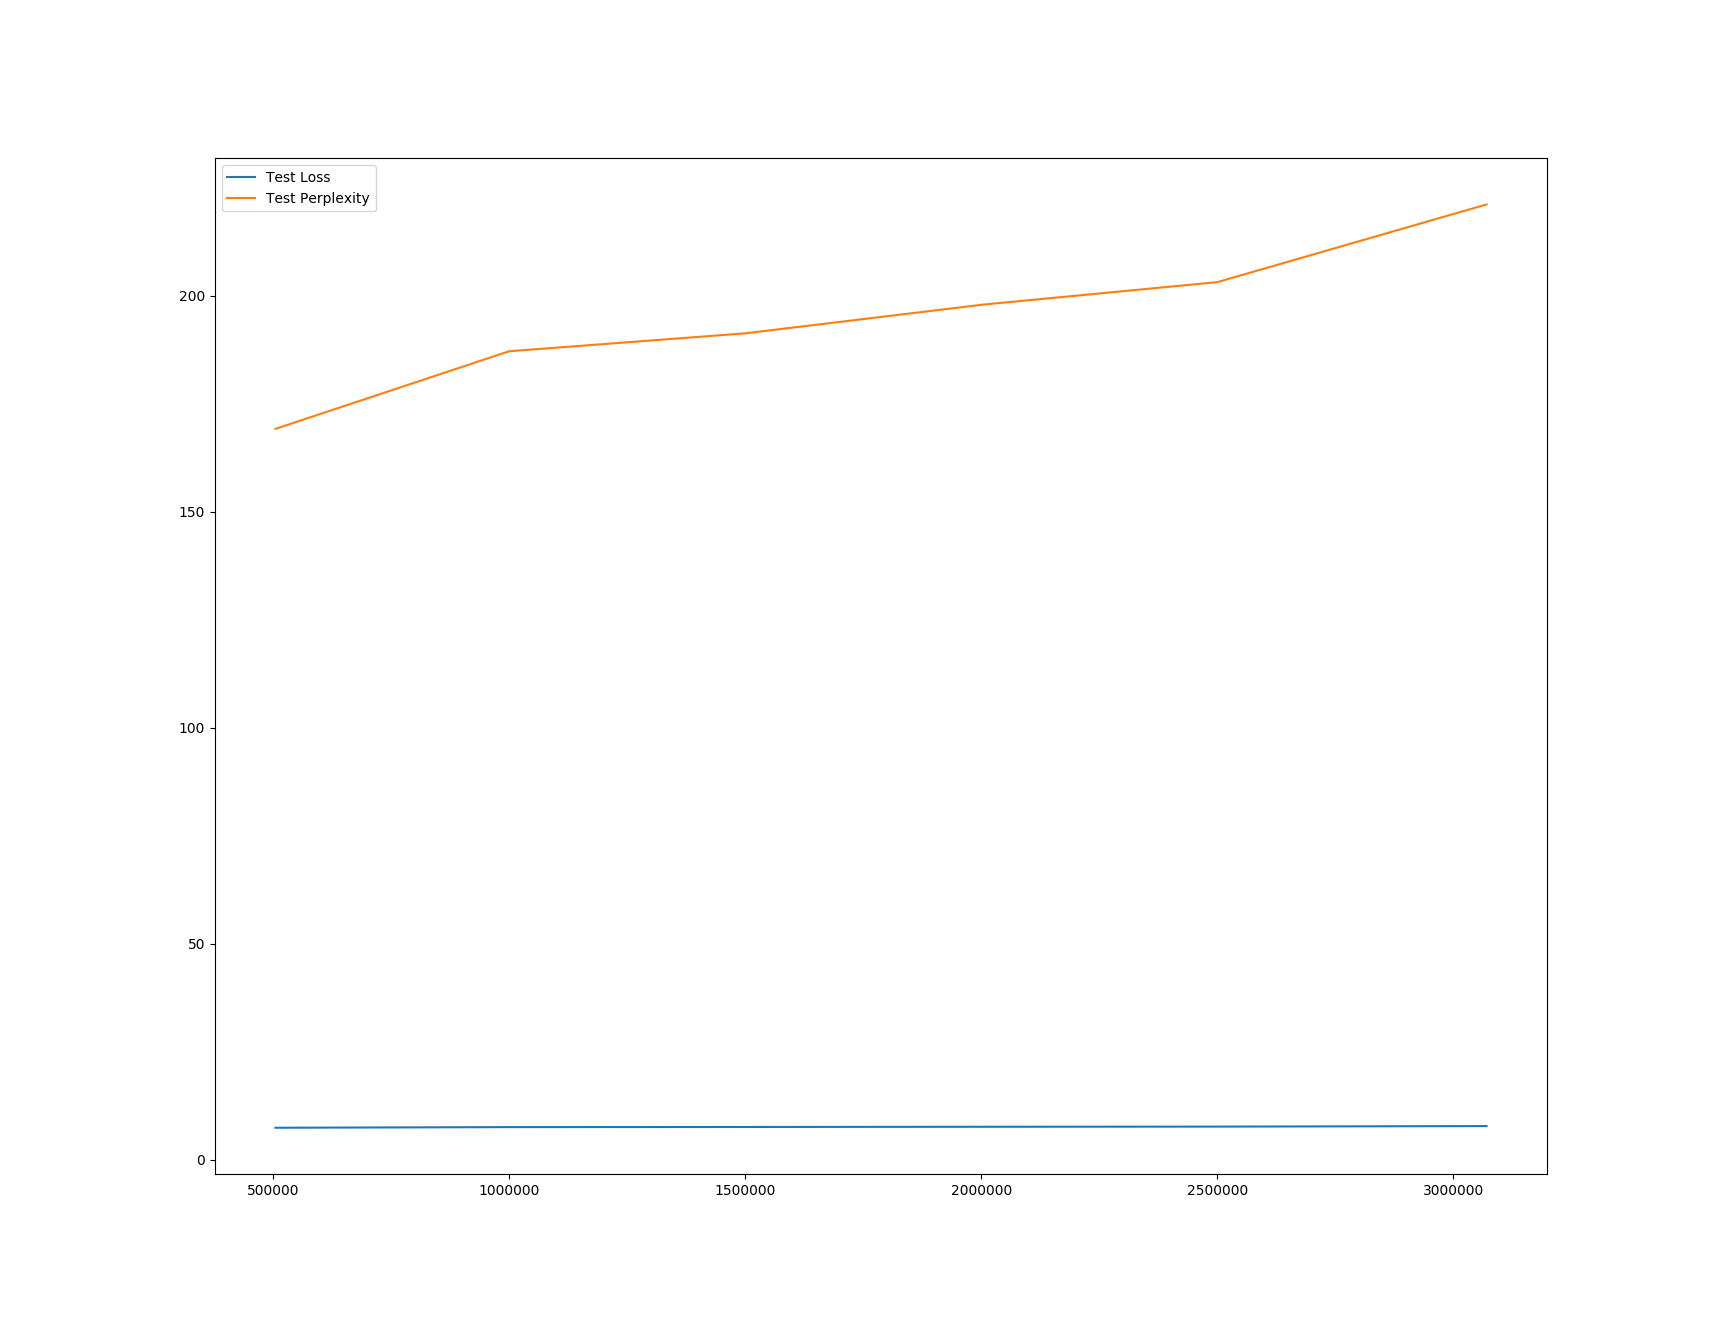
\includegraphics[width=\linewidth]{img/plots/reddit/test_metrics_both.png}
	\centering
	\small
	\text{The loss and perplexity.}
	\endminipage\hfill
	\minipage{0.5\textwidth}
	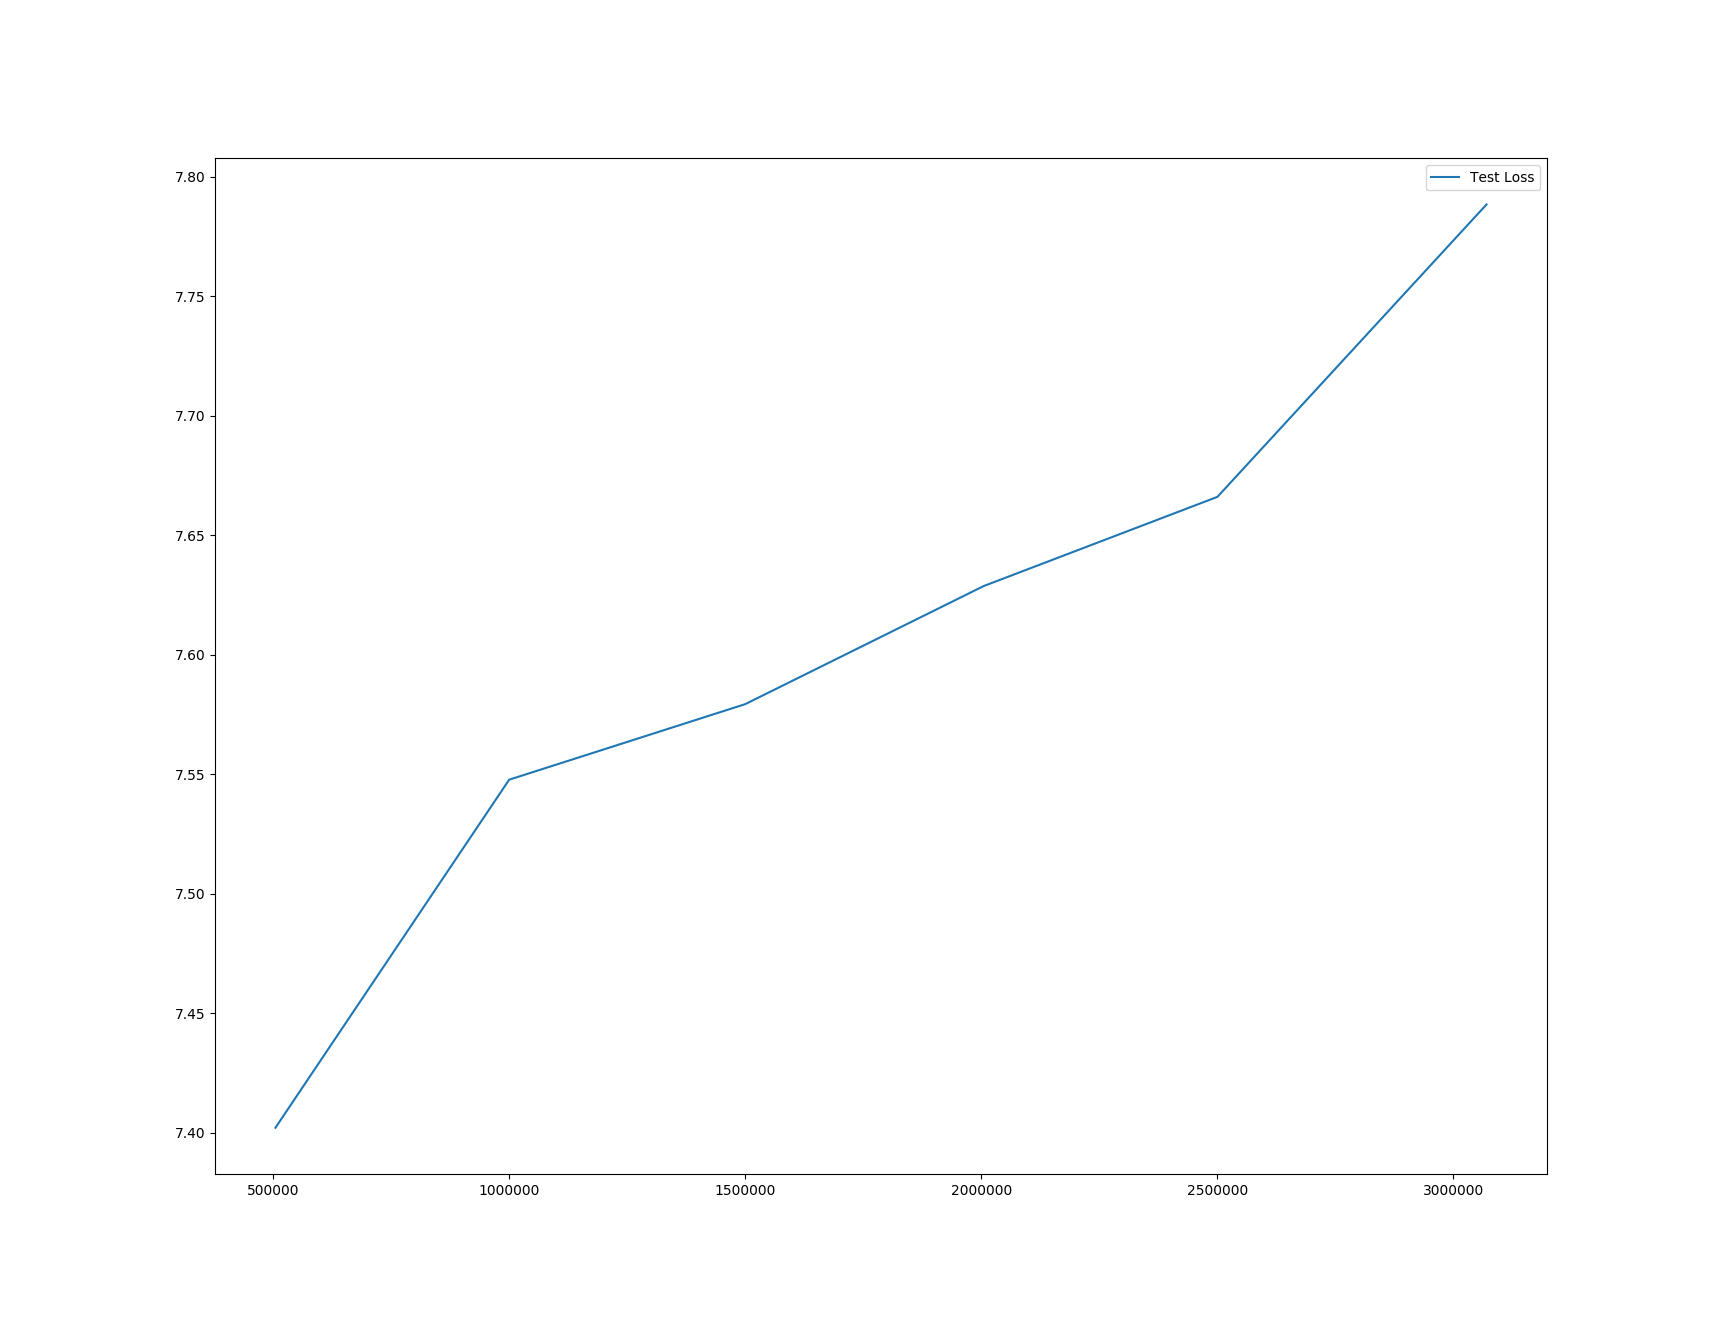
\includegraphics[width=\linewidth]{img/plots/reddit/test_metrics_loss.png}
	\centering
	\small
	\text{Only the loss.}
	\endminipage\hfill
	\caption{The loss and perplexity by running the six different snapshots against the test dataset using the Reddit model.}
	\label{result:test_performance:reddit}
\end{figure}

\paragraph{Progress Is Achieved}\todo{fuck title} As the results of evaluating the models on the test dataset has shown, it seems that the models did not make an meaningful progress throughout the training. For this reason, we decided that we would like to evaluate the model by hand and see if the generated responses improve when using the different six snapshots of the models. We opted for four different input sentences, that means two for each model, and generated responses for each of the snapshots. The results can be seen in the Table~\ref{results:example_output:reddit} for the Reddit model and Table~\ref{results:example_output:opensubtitles} for the OpenSubtitles model.

\begin{table}[H]
	\centering
	\ra{1.3}
	\begin{adjustbox}{max width=\textwidth}
		\begin{tabular}{ll}
			\toprule
			Input: 	& \texttt{Do you like Joffrey from game of thrones?}\\
			\midrule
			0.5M: 	& \texttt{i m not sure if you re a fan of the movie ,}\\
			& \texttt{but i m not sure if you re a fan of the movie .}\\
			1.0M: 	& \texttt{i m not a fan of the game , but i m not sure if it s a game or not .}\\
			1.5M:	& \texttt{i do nt know what i m talking about .}\\
			2.0M:	& \texttt{i do nt }\\
			2.5M:	& \texttt{i do nt know what i m talking about .}\\
			3.0M:	& \texttt{i do nt know , i just do nt like him .}\\
			\midrule
			Input: 	& \texttt{Which movie can you recommend me?}\\
			\midrule
			0.5M: 	& \texttt{the}\\
			1.0M: 	& \texttt{the movie .}\\
			1.5M:	& \texttt{the one with the}\\
			2.0M:	& \texttt{the dark knight rises}\\
			2.5M:	& \texttt{the prestige}\\
			3.0M:	& \texttt{the movie}\\
			\bottomrule
		\end{tabular}
	\end{adjustbox}
	\caption{Two example dialogs with the Reddit model with one response per snapshot.}
	\label{results:example_output:reddit}
\end{table}
\todo{Format so that all look the same, probably by using tabularx and an X column}

\begin{table}[H]
	\centering
	\ra{1.3}
	\begin{adjustbox}{max width=\textwidth}
		\begin{tabular}{ll}
			\toprule
			Input: 	& \texttt{Are you a man or a woman?}\\
			\midrule
			0.5M: 	& \texttt{no , no , no}\\
			1.0M: 	& \texttt{no}\\
			1.5M:	& \texttt{i m not a man}\\
			2.0M:	& \texttt{i m not a woman}\\
			2.5M:	& \texttt{i m a man}\\
			3.0M:	& \texttt{i m not a woman}\\
			\midrule
			Input: 	& \texttt{Why should it not be a good idea to improve you?}\\
			\midrule
			0.5M: 	& \texttt{no}\\
			1.0M: 	& \texttt{i don t know}\\
			1.5M:	& \texttt{because i love you}\\
			2.0M:	& \texttt{because i m a good man}\\
			2.5M:	& \texttt{i m just trying to make a good decision}\\
			3.0M:	& \texttt{i m not a good idea}\\
			\bottomrule
		\end{tabular}
	\end{adjustbox}
	\caption{Two example dialogs with the OpenSubtitles model with one response per snapshot.}
	\label{results:example_output:opensubtitles}
\end{table}

As seen in the examples above, there has indeed been an improvement in the answers, what stands in contradiction to the development of the performance of the models on the test datasets. Our conclusion from this is, again, that the cross-entropy loss and perplexity are not fit to asses if the responses are meaningful.\todo{Write more?} As we have already described in Chapter~\ref{fundamentals:sent2vec_test}, we were aware of the fact, that our current set of metrics is not satisfying for evaluating if the responses are meaningful, why we decided to use yet another metric, namely Sent2Vec embeddings, which we are going to use in the next section.

\paragraph{Sent2Vec Analysis} As described in Chapter~\ref{fundamentals:sent2vec_test}, we use Sent2Vec embeddings for measuring the semantic similarity between the generated and expected responses on the test dataset. For this purpose, we have used the pretrained models available on the GitHub page of the project\footnote{https://github.com/epfml/sent2vec}. We have decided, that we use both the \emph{Twitter} and \emph{Wikipedia} models for the assessment. The results can be seen in the Figures~\ref{results:sent2vec:opensubtitles:results} and~\ref{results:sent2vec:reddit:results}. What can be directly seen is that both the Reddit and OpenSubtitles models perform better on the pretrained Wikipedia model in comparison to the pretrained twitter model. This probably has to do with the fact that ``compressed'' language used when writing tweets (e.g. ``w/o'' instead of ``without'') and with the coverage of the vocabulary, which is higher with the Wikipedia model.\todo{Need to check that!} However, both results are pretty bad, with the Reddit results being much better than the OpenSubtitles, about twice as good (see Tables~\ref{results:sent2vec:opensubtitles:results_table} and~\ref{results:sent2vec:reddit:results_table}). The OpenSubtitles model starts with an average similarity of $0.167$ for the first snapshot and climbs up to $0.204$ for the last snapshot. The Reddit model starts with an average value of $0.336$ for the first snapshot and increases to $0.359$ for the last snapshot. This means, that the responses of the Reddit model match the expected responses much better from a semantic perspective as the responses of the OpenSubtitles model do. In summary, the results of both models are pretty bad, as the maximum similarity is $1.0$.\todo{Write, or remove that?}

\begin{figure}[H]
	\minipage{0.5\textwidth}
	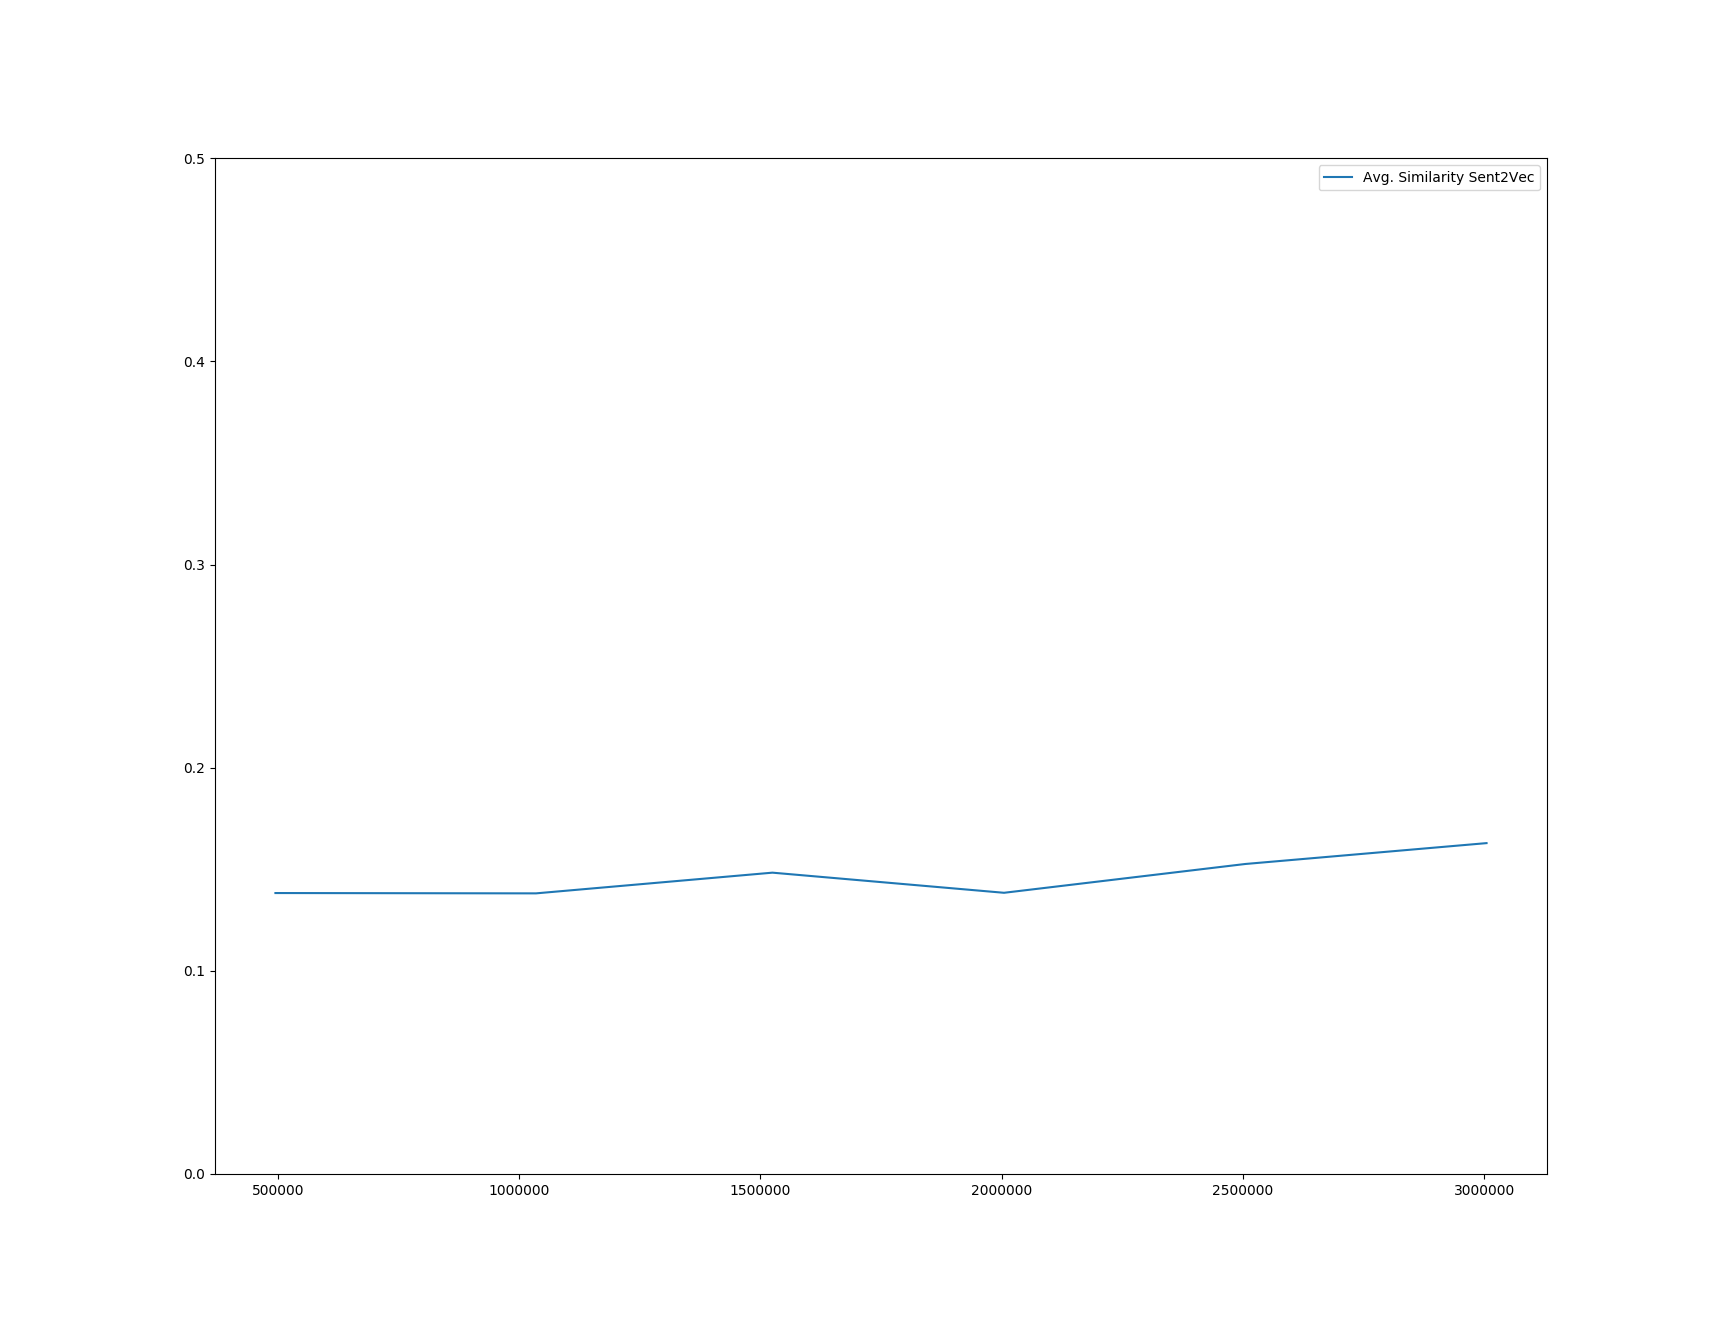
\includegraphics[width=\linewidth]{img/plots/opensubtitles_not_reversed/s2v_wiki_cosine_similarity.png}
	\centering
	\small
	\text{Wikipedia}
	\endminipage\hfill
	\minipage{0.5\textwidth}
	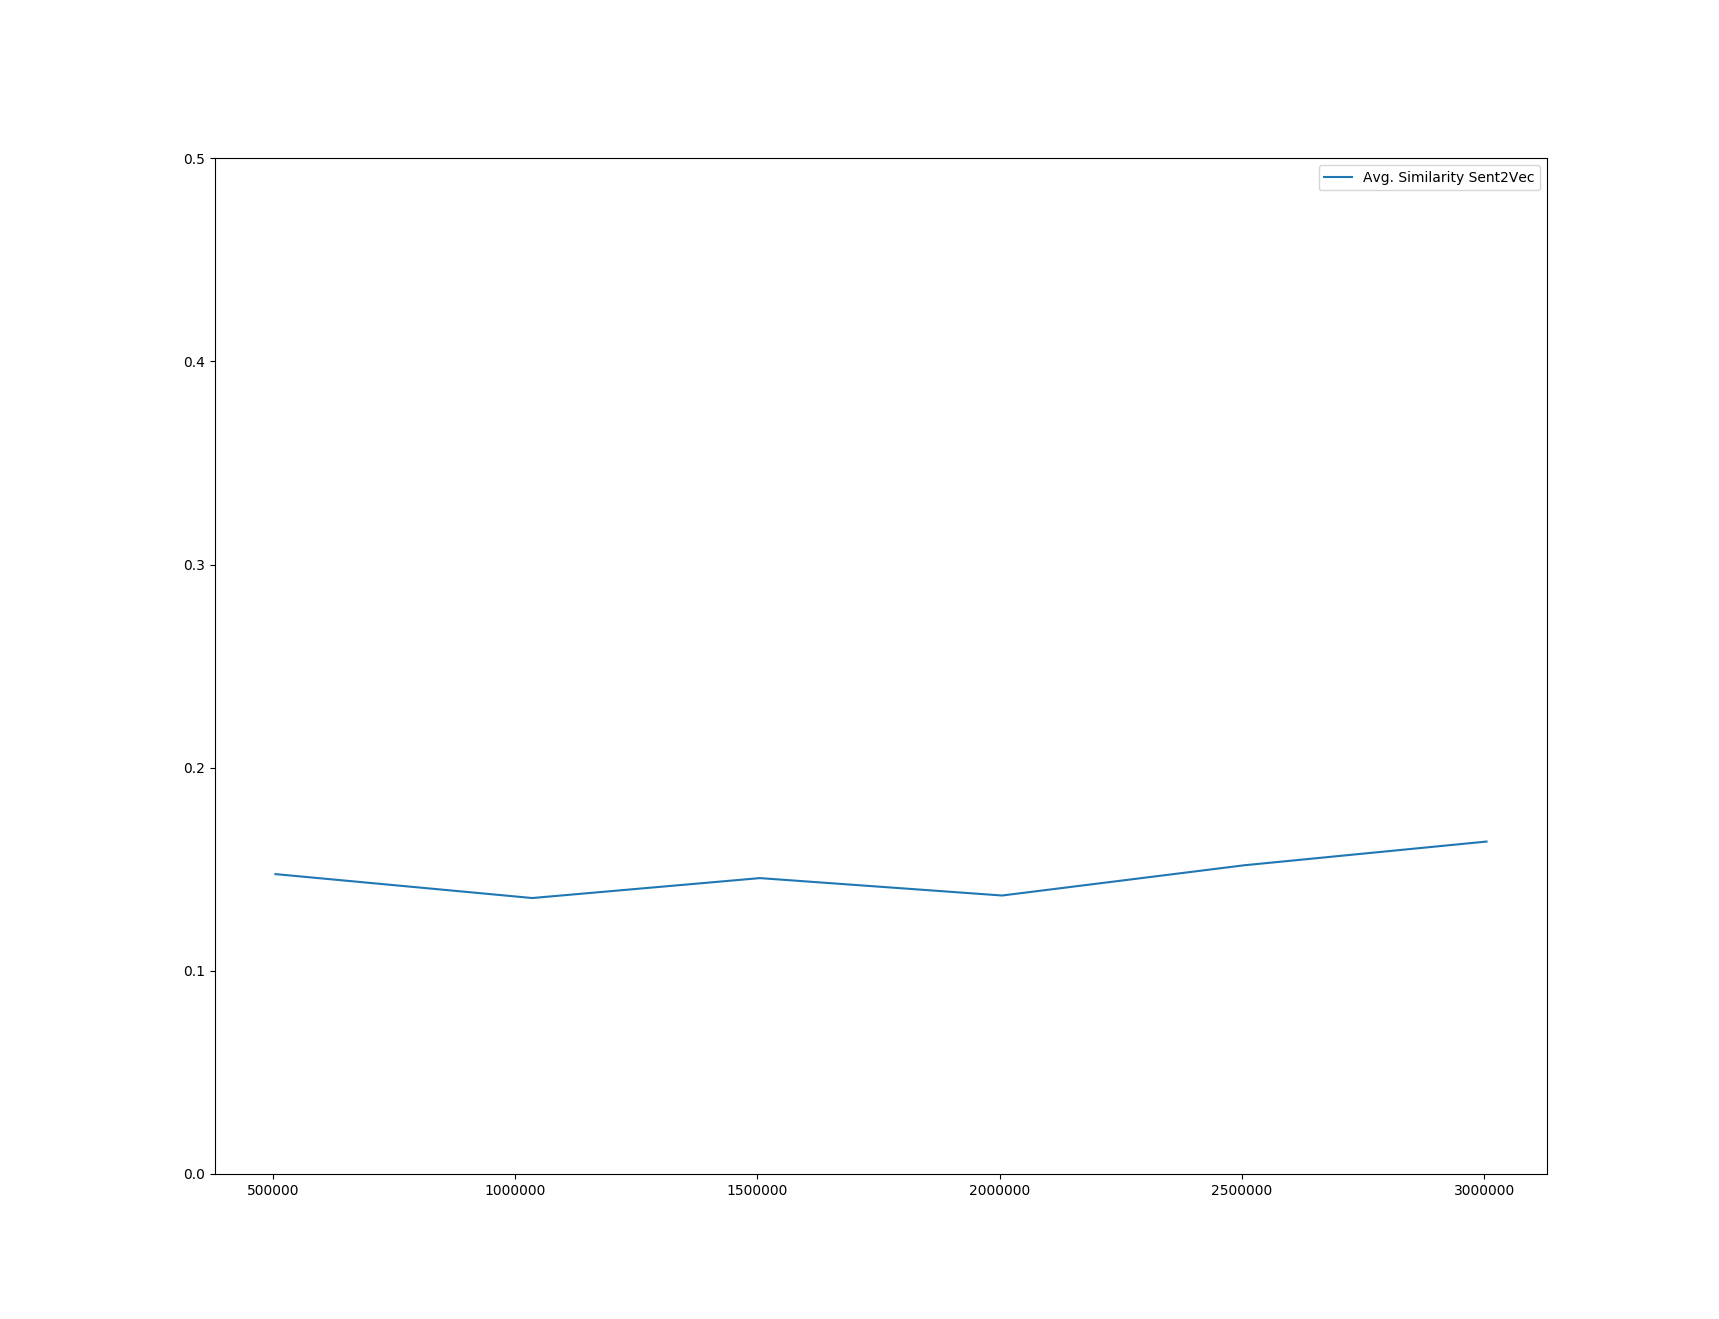
\includegraphics[width=\linewidth]{img/plots/opensubtitles_not_reversed/s2v_twitter_cosine_similarity.png}
	\centering
	\small
	\text{Twitter}
	\endminipage\hfill
	\caption{Results of the evaluation with Sent2Vec on the outputs of the OpenSubtitles models using the pretrained models. The ticks on the x-axis show the different snapshots and the y-axis the average semantic similarity when using Sent2Vec for each snapshot.}
	\label{results:sent2vec:opensubtitles:results}
\end{figure}

\begin{table}[H]
	\centering
	\ra{1.3}
	\begin{adjustbox}{max width=\textwidth}
		\begin{tabular}{lcc}
			\toprule
			Snapshot & Avg. Similarity (Wikipedia) & Avg. Similarity (Twitter)\\
			\midrule
			0.5M & $0.16749$ & $0.13827$\\
			1.0M & $0.19111$ & $0.13811$\\
			1.5M & $0.19418$ & $0.14831$\\
			2.0M & $0.19176$ & $0.13840$\\
			2.5M & $0.20118$ & $0.15258$\\
			3.0M & $0.20452$ & $0.16285$\\
			\bottomrule
		\end{tabular}
	\end{adjustbox}
	\caption{The average similarities when applying the Sent2Vec metric on the expected and generated responses from the OpenSubtitles model.}
	\label{results:sent2vec:opensubtitles:results_table}
\end{table}

\begin{figure}[H]
	\minipage{0.5\textwidth}
	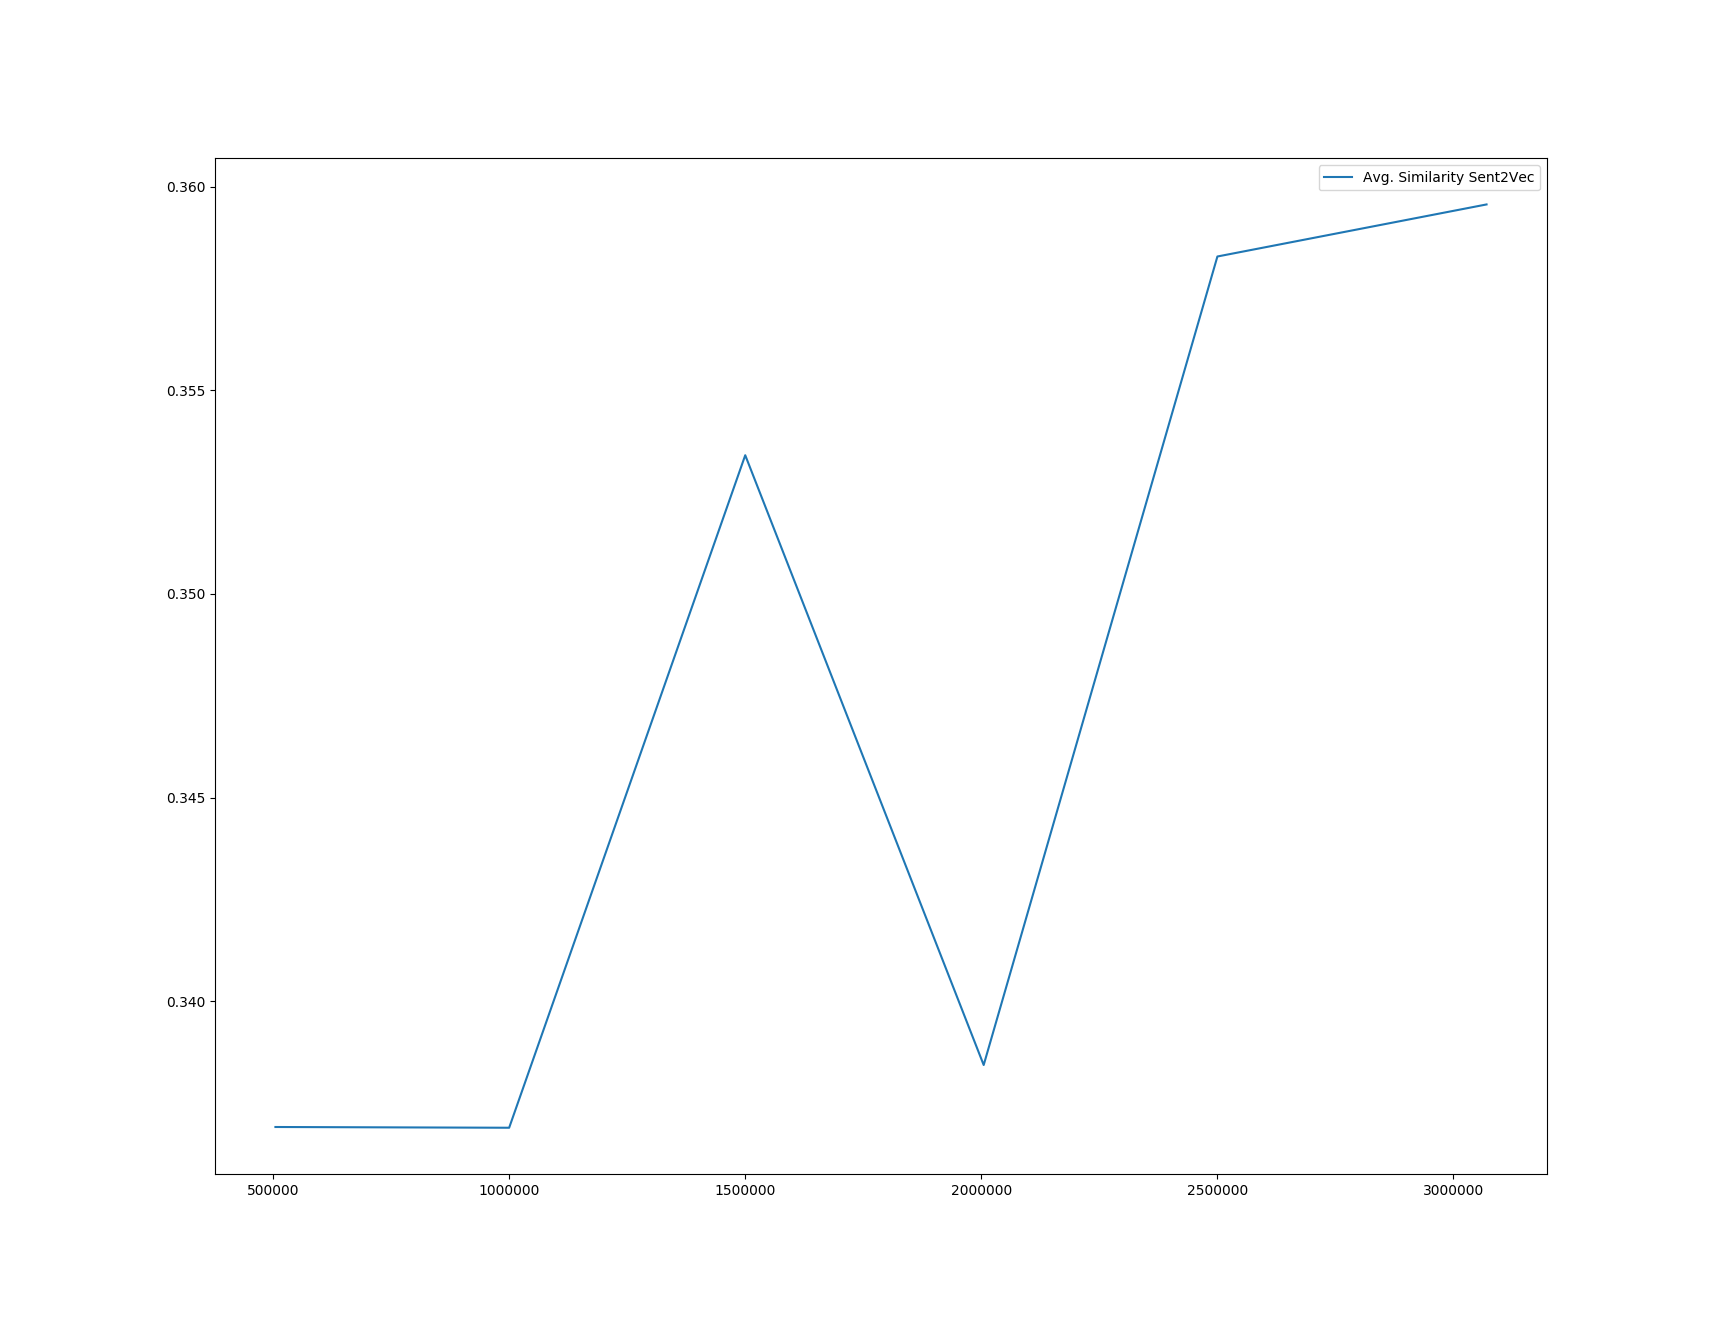
\includegraphics[width=\linewidth]{img/plots/reddit/s2v_wiki_cosine_similarity.png}
	\centering
	\small
	\text{Wikipedia}
	\endminipage\hfill
	\minipage{0.5\textwidth}
	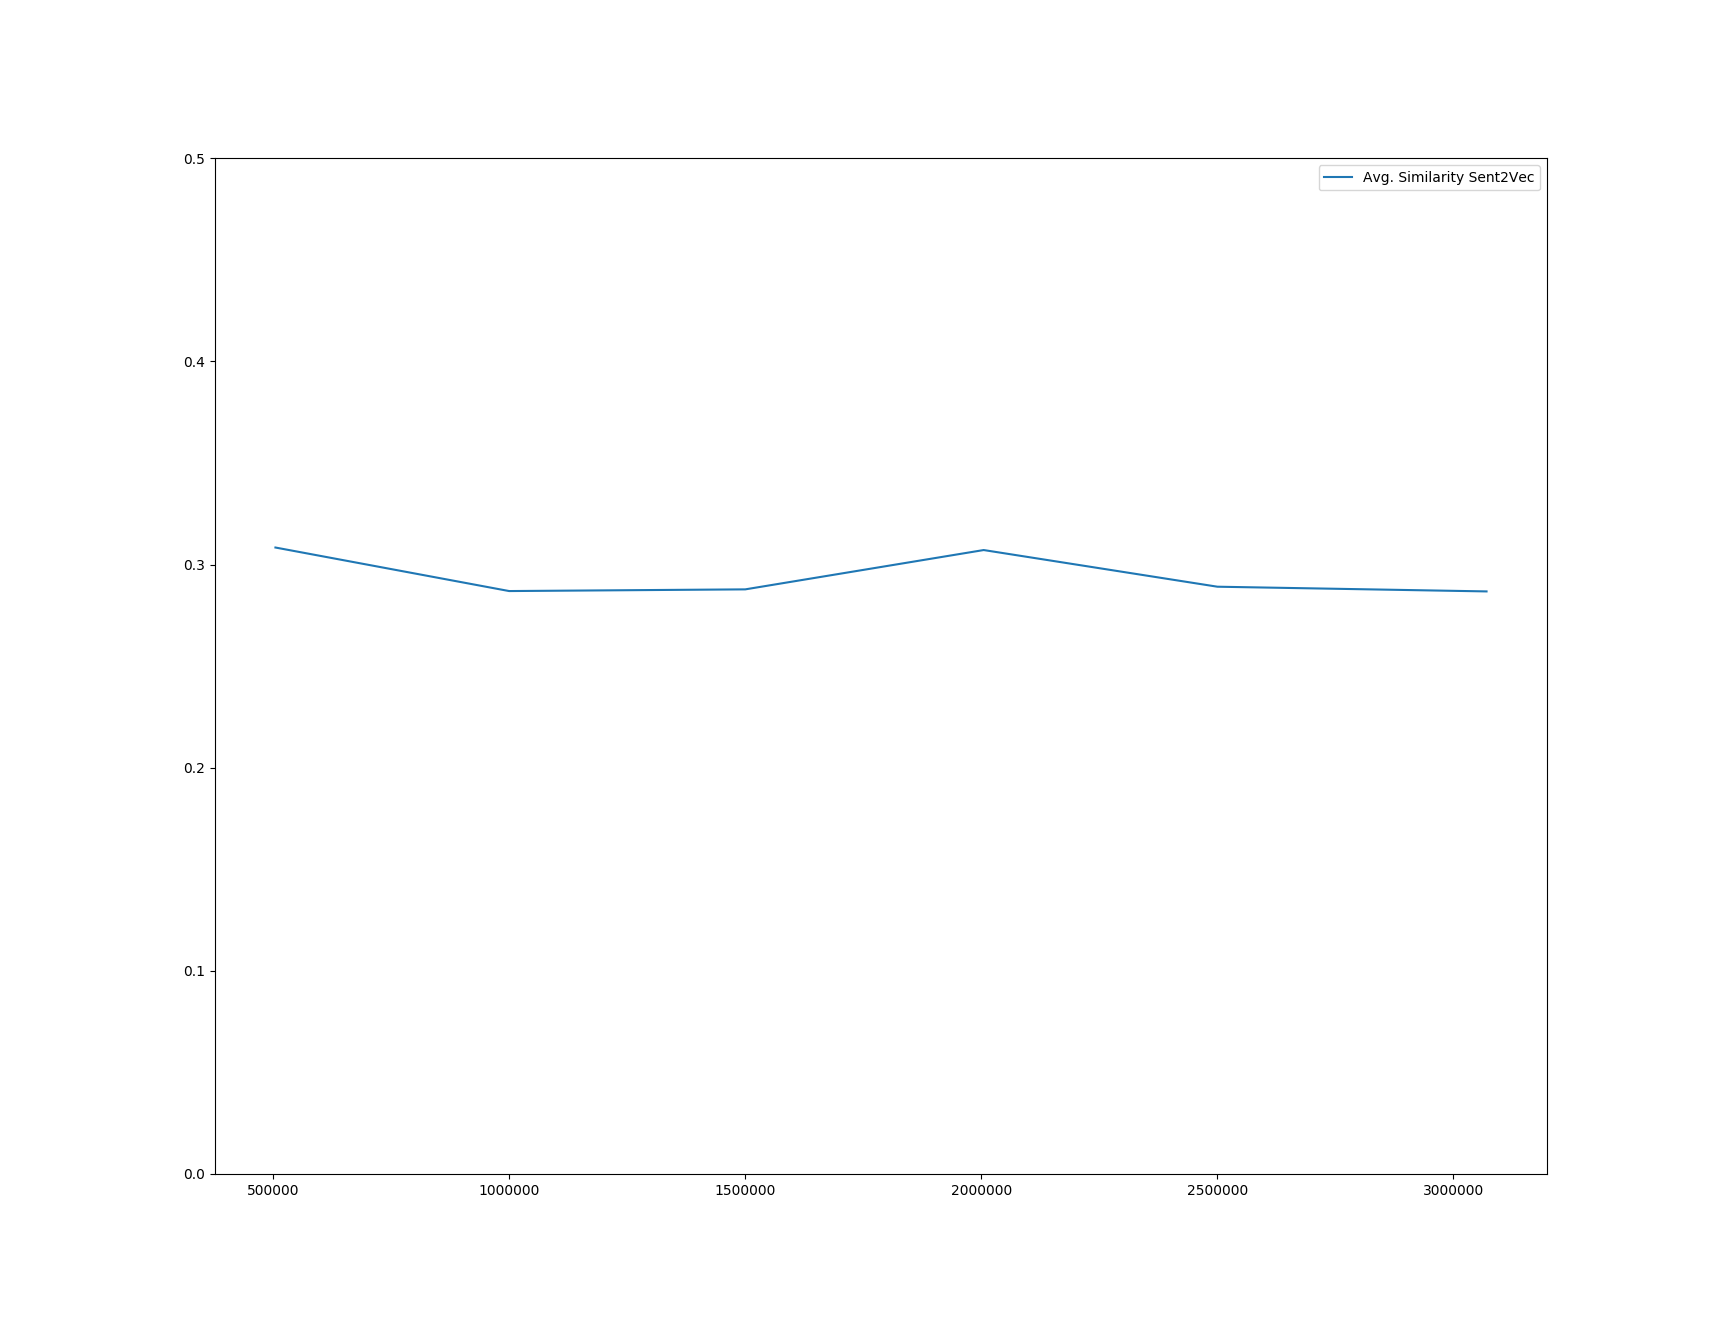
\includegraphics[width=\linewidth]{img/plots/reddit/s2v_twitter_cosine_similarity.png}
	\centering
	\small
	\text{Twitter}
	\endminipage\hfill
	\caption{Results of the evaluation with Sent2Vec on the outputs of the Reddit models using the pretrained models. The ticks on the x-axis show the different snapshots and the y-axis the average semantic similarity when using Sent2Vec for each snapshot.}
	\label{results:sent2vec:reddit:results}
\end{figure}
\begin{table}[H]
	\centering
	\ra{1.3}
	\begin{adjustbox}{max width=\textwidth}
		\begin{tabular}{lcc}
			\toprule
			Snapshot & Avg. Similarity (Wikipedia) & Avg. Similarity (Twitter)\\
			\midrule
			0.5M & $0.33691$ & $0.30837$\\
			1.0M & $0.33689$ & $0.28694$\\
			1.5M & $0.35340$ & $0.28777$\\
			2.0M & $0.33843$ & $0.30713$\\
			2.5M & $0.35828$ & $0.28908$\\
			3.0M & $0.35956$ & $0.28676$\\
			\bottomrule
		\end{tabular}
	\end{adjustbox}
	\caption{The average similarities when applying the Sent2Vec metric on the expected and generated responses from the Reddit model.}
	\label{results:sent2vec:reddit:results_table}
\end{table}

\todo{Fazit for this paragraph?}

\paragraph{Generic Response are a Problem} One potential reason for the bad results when using the Sent2Vec metric is that we witnessed both models generating generic responses a lot of the time. To analyze this our first idea was to see, what kind of sentences the models produce with the inputs of the test datasets. We did an analysis on the generated responses and quickly noticed that there are a few sentences, which the models predict a lot of time (see Tables~\ref{results:test_performance:opensubtitles_sample_outputs} and~\ref{results:test_performance:reddit_sample_outputs}).
\\
\begin{table}[H]
	\centering
	\ra{1.3}
	\begin{adjustbox}{max width=\textwidth}
		\begin{tabular}{ll}
			\toprule
			Sentence & Frequency\\ \midrule
			\texttt{i m not gon na let you go} & 41853\\
			\texttt{i m not sure i can trust you} & 21263\\
			\texttt{i m not gon na say anything} & 9163\\
			\texttt{i m not gon na let that happen} & 7426\\
			\texttt{i m sorry} & 7235\\
			\texttt{you re not gon na believe this} & 7068\\
			\texttt{you re not gon na believe me} & 6878\\
			\texttt{i m not gon na hurt} you & 4829\\
			\texttt{i m not a fan} & 4468\\
			\texttt{i m not sure} & 4215\\
			\bottomrule
		\end{tabular}
	\end{adjustbox}
	\caption{Top 10 most generated responses with respective occurence frequencies when using the last OpenSubtitles snapshot on the test dataset.}
	\label{results:test_performance:opensubtitles_sample_outputs}
\end{table}\todo{Totale Anzahl sätze angeben? (können wir ja berechnen?)}\todo{make tables the same width!}

\begin{table}[H]
	\centering
	\ra{1.3}
	\begin{adjustbox}{max width=\textwidth}
		\begin{tabular}{ll}
			\toprule
			Sentence & Frequency\\ \midrule
			\texttt{i m not sure if i m being sarcastic or not .} & 17486\\
			\texttt{i think it s a bit of a stretch .} & 13058\\
			\texttt{i m not sure if you re being sarcastic or not .} & 11647\\
			\texttt{i m not sure if i m a <unknown> or not .} & 8307\\
			\texttt{i m not sure if you re joking or not .} & 7932\\
			\texttt{i was thinking the same thing .} & 7579\\
			\texttt{<unknown>} & 6210\\
			\texttt{i m not sure if i m going to watch this or not .} & 4257\\
			\specialcell{\texttt{i m not sure if i m a fan of the show , but i m}\\\texttt{pretty sure that s a <unknown> .}} & 3232\\
			\texttt{i m not sure if i m going to watch it or not .} & 3079\\
			\bottomrule
		\end{tabular}
	\end{adjustbox}
	\caption{Top 10 most generated sentences with respective occurence frequencies when using the last Reddit snapshot on the test dataset.}
	\label{results:test_performance:reddit_sample_outputs}
\end{table}\todo{Totale Anzahl sätze angeben? (können wir ja berechnen?)}\todo{make tables the same width!}

 \todo{Table for results of sent2vec analysis}

As seen in the both tables above, there are certain responses which are generated a lot of time and are pretty generic and meaningless. Because of that, we thought it would be a good idea to evaluate the models under the Sent2Vec metric one more time, but this time with the top $n$ generic sentences filtered out. We did this with the hope that the generic sentences are the cause of the small average similarity. The results of the analysis with the top $n$ sentences filtered out can be found in Table~\ref{results:sent2vec:opensubtitles:top_n_results_table} and~\ref{results:sent2vec:reddit:top_n_results_table}. For this analysis, we have only used the Wikipedia model as it has shown a better performance for both of our models before.
\\
\begin{table}[H]
	\centering
	\ra{1.3}
	\begin{adjustbox}{max width=\textwidth}
		\begin{tabular}{lccc}
			\toprule
			Snapshot & $n = 1$ & $n = 5$ & $n = 10$\\
			\midrule
			0.5M & $0.16679$ & $0.16804$ & $0.16854$\\
			1.0M & $0.19329$ & $0.19394$ & $0.19575$\\
			1.5M & $0.19491$ & $0.19519$ & $0.19539$\\
			2.0M & $0.19215$ & $0.19192$ & $0.19284$\\
			2.5M & $0.20102$ & $0.20127$ & $0.20182$\\
			3.0M & $0.20431$ & $0.20547$ & $0.20568$\\
			\bottomrule
		\end{tabular}
	\end{adjustbox}
	\caption{The average similarities when applying the Sent2Vec metric on the expected and generated responses on the test dataset when filtering out the top $n$ most generated responses the OpenSubtitles model.}
	\label{results:sent2vec:opensubtitles:top_n_results_table}
\end{table}

\begin{table}[H]
	\centering
	\ra{1.3}
	\begin{adjustbox}{max width=\textwidth}
		\begin{tabular}{lccc}
			\toprule
			Snapshot & $n = 1$ & $n = 5$ & $n = 10$\\
			\midrule
			0.5M & $0.33772$ & $0.34101$ & $0.34589$\\
			1.0M & $0.34225$ & $0.34238$ & $0.34295$\\
			1.5M & $0.35383$ & $0.35605$ & $0.35564$\\
			2.0M & $0.34008$ & $0.34009$ & $0.34198$\\
			2.5M & $0.35937$ & $0.36142$ & $0.36175$\\
			3.0M & $0.36043$ & $0.35950$ & $0.36313$\\
			\bottomrule
		\end{tabular}
	\end{adjustbox}
	\caption{The average similarities when applying the Sent2Vec metric on the expected and generated responses on the test dataset when filtering out the top $n$ most generated responses for the Reddit model.}
	\label{results:sent2vec:reddit:top_n_results_table}
\end{table}

As seen in the tables above, the filtering of the most used responses does not help a lot when it comes to the Sent2Vec evaluation.

\paragraph{Mixed Feelings about Performance Metrics} As seen in this chapter, the performance metrics used to evaluate the models tell us a mixed story about the resulting models. On one hand, we see that the training went fine and the learning process run as expected. However, when we then test these trained models against the test datasets with the different metrics, it looks like the performance got worse and worse over the time of the training. This is not true in our subjective opinion after ``talking'' to both models for a prolonged period of time. We think the biggest problem for the evaluation are the generic responses both models seem to generate much more than actual answers. To find the cause of this generic responses, we will now try to analyze the language model which both models have learned while training and try to establish a connection between the language model in the datasets and the ones produced by the models.

\section{Language Model \& Semantic Understanding}
As said at the end of the previous chapter, in this chapter we are going to investigate into the language models the trained models produce and try to get a grasp on how much semantic understanding the models have. For the first analysis, we are going to create compare n-gram distributions over the datasets and compare them with the distributions found in the responses when evaluating the models. We also take a look at the most use n-grams to find a reason why the models produce so much generic sentences. After that, we are going to investigate into how the models actually process the input sequences by first taking a look at the generated thought vectors. We will then go on and try to evaluate if the attention mechanism (see Chapter~\ref{fundamentals:soft_attention}) really helps the models when producing responses.

\paragraph{Uni- and Bigram Distributions over Time}
As the first step, we are going to compare the uni- and bigram distributions of the training datasets with the distributions produced when evaluating the models with the test datasets. For this purpose, we generated unigram and bigram statistics using \texttt{nltk} over the training datasets and outputs generated by the models. First, let us analyze the bigram distributions which can be seen in the Figures~\ref{results:bigram:distributions:opensubtitles} and~\ref{results:bigram:distributions:reddit}. As seen there, at the beginning of the training (i.e. snapshots 0.5M), the bigrams are distributed pretty evenly. However, as longer as the training continues the more right-leaning the distributions of the bigrams in the outputs of the models get. This seems to coincide with the results found in the previous chapter, that the models start to use less and less bigrams but simultaneously increases the usage frequency of often used bigrams. It is also understandable from a stand point that the models learn, which are the important bigrams and which are not. This is especially apparent in the case of the OpenSubtitles model, where we also witness a big discrepancy between the expected and the generated distributions. However, the development of the distribution in the case of the Reddit model looks quite different. It also becomes more right-leaning as the training advances, but it much better fits the expected distribution, for example bigrams in the snapshot 1.5M have almost the same distribution as in the training data.

\begin{figure}[H]
	\minipage{0.5\textwidth}
	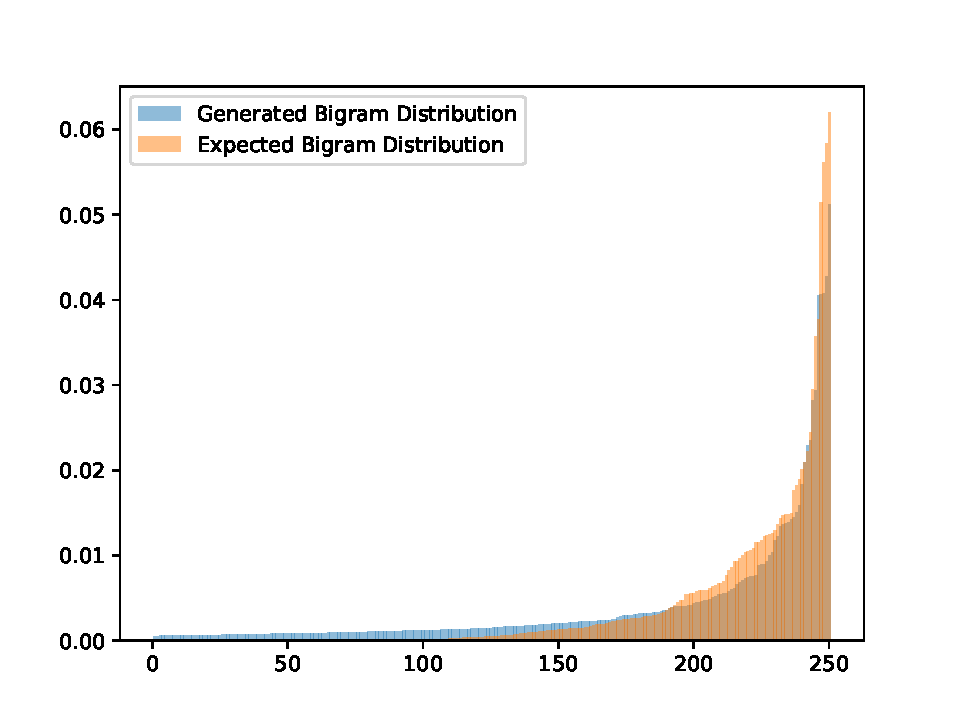
\includegraphics[width=\linewidth]{img/plots/opensubtitles_not_reversed/bigram_distribution_comparison_step_500000.pdf}
	\centering
	\small
	\text{Snapshot 0.5M}
	\endminipage\hfill
	\minipage{0.5\textwidth}
	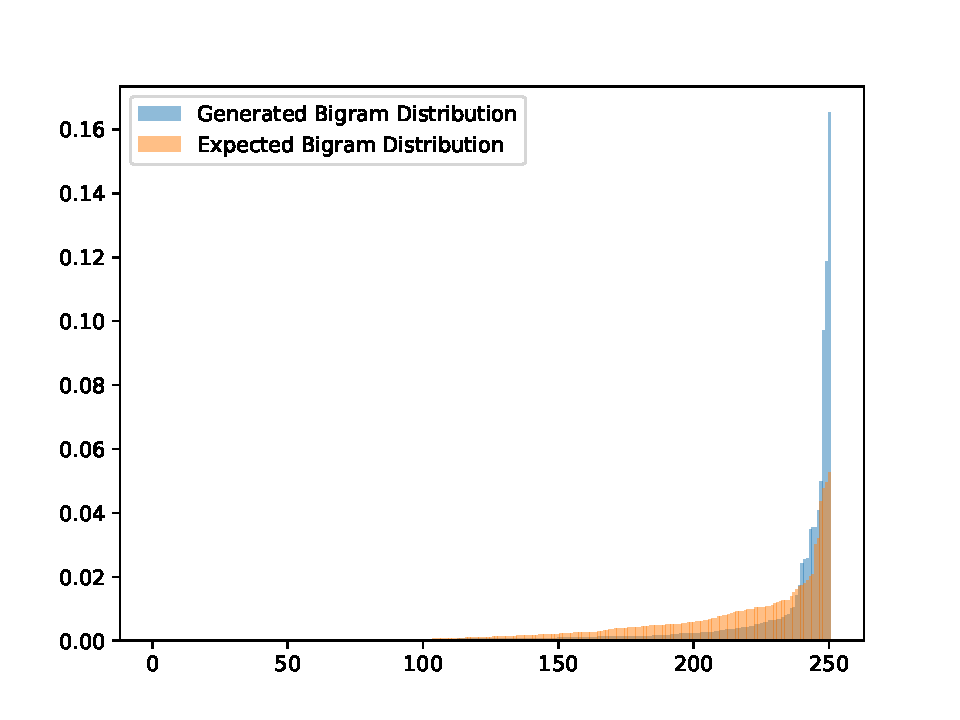
\includegraphics[width=\linewidth]{img/plots/opensubtitles_not_reversed/bigram_distribution_comparison_step_1000000.pdf}
	\centering
	\small
	\text{Snapshot 1.0M}
	\endminipage\hfill
	\minipage{0.5\textwidth}
	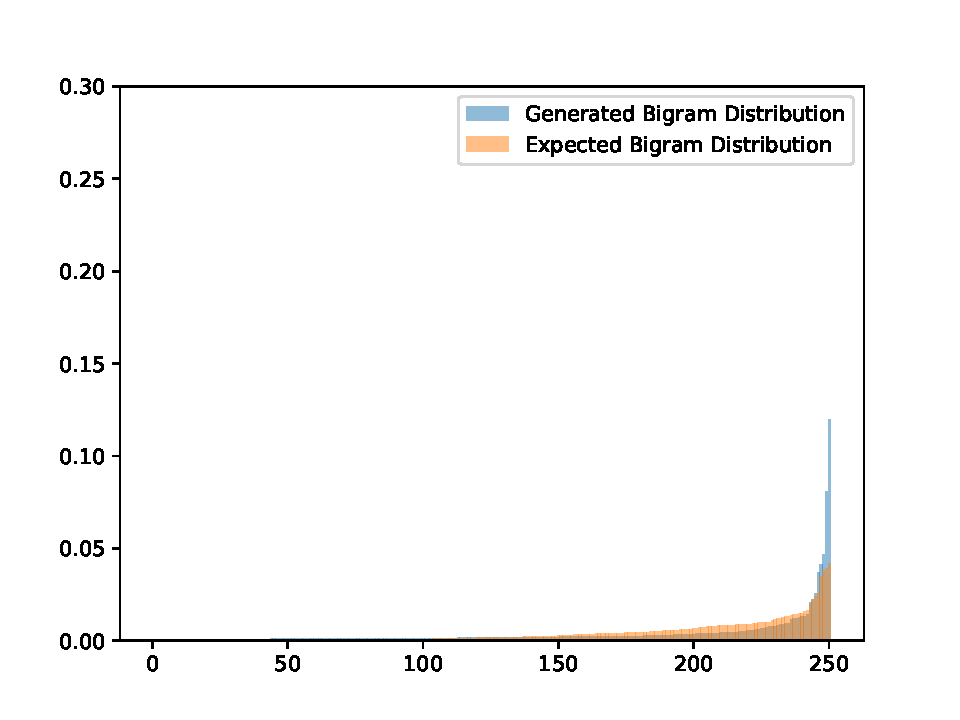
\includegraphics[width=\linewidth]{img/plots/opensubtitles_not_reversed/bigram_distribution_comparison_step_1500000.pdf}
	\centering
	\small
	\text{Snapshot 1.5M}
	\endminipage\hfill
	\minipage{0.5\textwidth}
	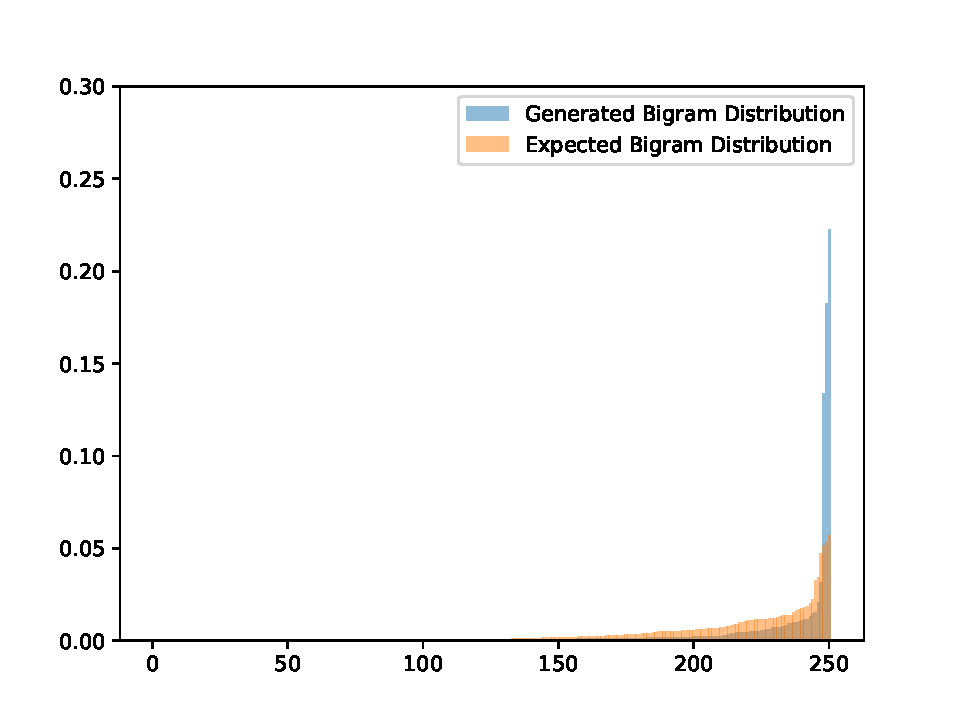
\includegraphics[width=\linewidth]{img/plots/opensubtitles_not_reversed/bigram_distribution_comparison_step_2000000.pdf}
	\centering
	\small
	\text{Snapshot 2.0M}
	\endminipage\hfill
	\minipage{0.5\textwidth}
	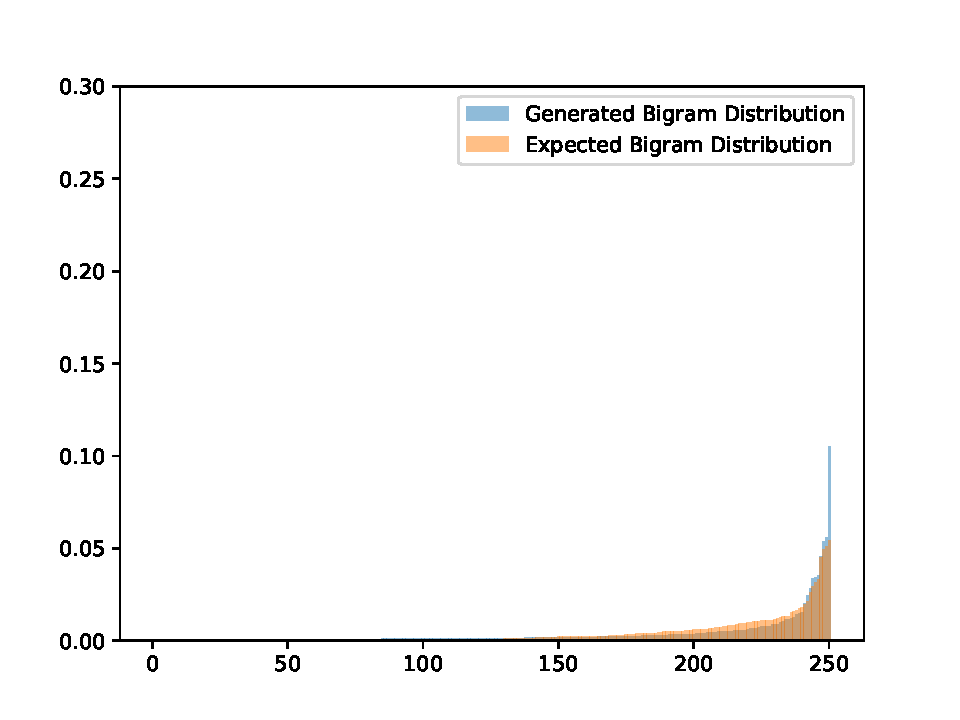
\includegraphics[width=\linewidth]{img/plots/opensubtitles_not_reversed/bigram_distribution_comparison_step_2500000.pdf}
	\centering
	\small
	\text{Snapshot 2.5M}
	\endminipage\hfill
	\minipage{0.5\textwidth}
	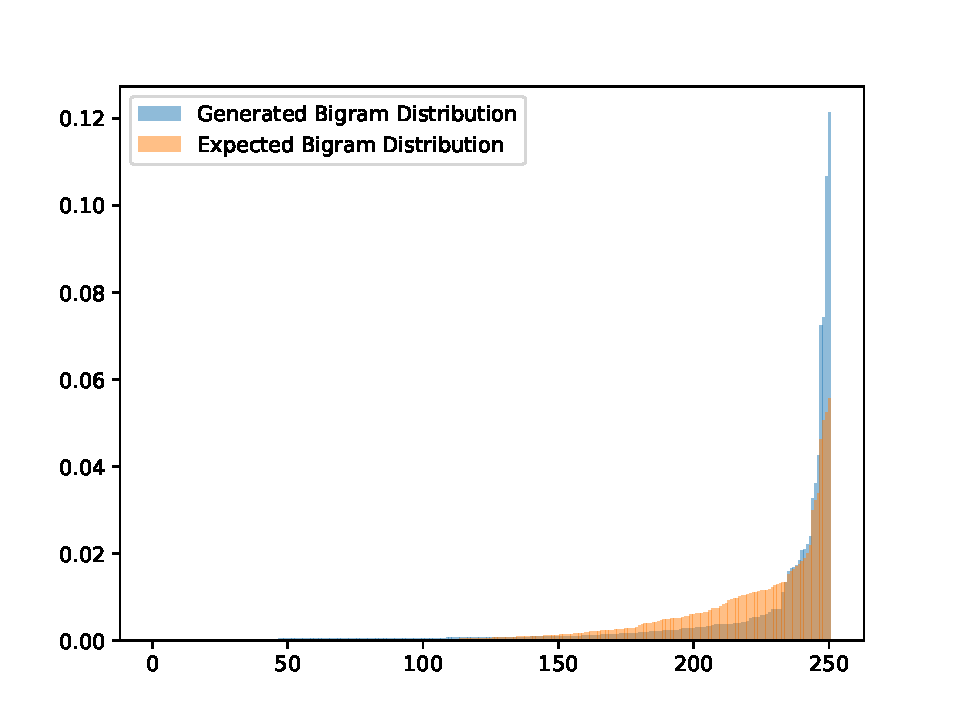
\includegraphics[width=\linewidth]{img/plots/opensubtitles_not_reversed/bigram_distribution_comparison_step_3000000.pdf}
	\centering
	\small
	\text{Snapshot 3.0M}
	\endminipage\hfill
	\caption{Comparison of the distributions of the top 100 most used bigrams for the responses of the OpenSubtitles models (orange) when using the test dataset and the distribution within the training data (blue). The distributions are compared for each snapshot available.}
	\label{results:bigram:distributions:opensubtitles}
\end{figure}

\begin{figure}[H]
	\minipage{0.5\textwidth}
	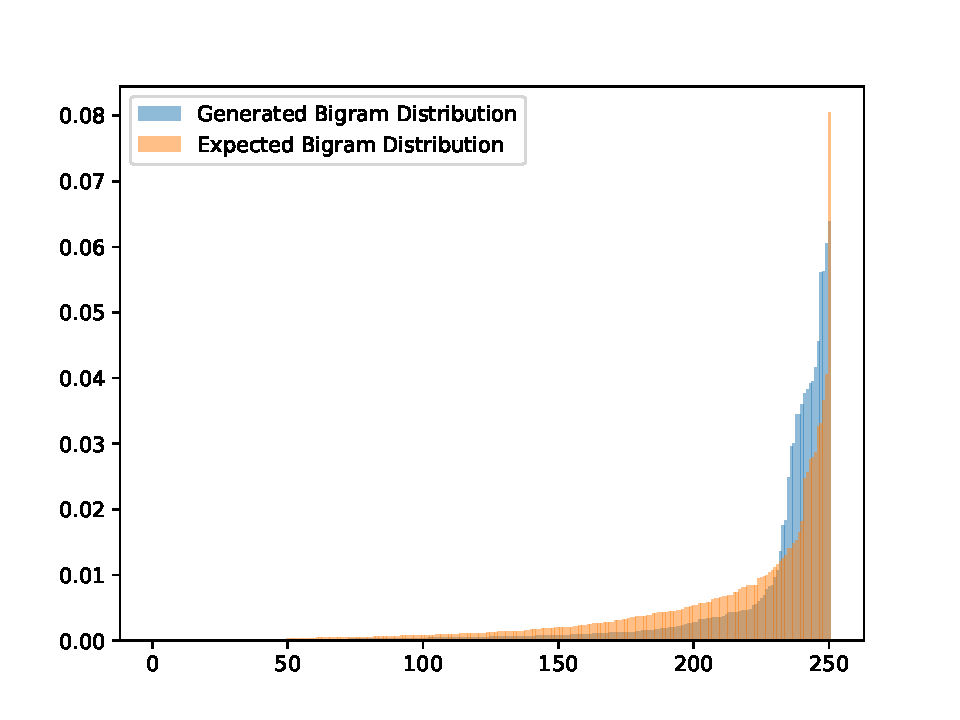
\includegraphics[width=\linewidth]{img/plots/reddit/bigram_distribution_comparison_step_500000.pdf}
	\centering
	\small
	\text{Snapshot 0.5M}
	\endminipage\hfill
	\minipage{0.5\textwidth}
	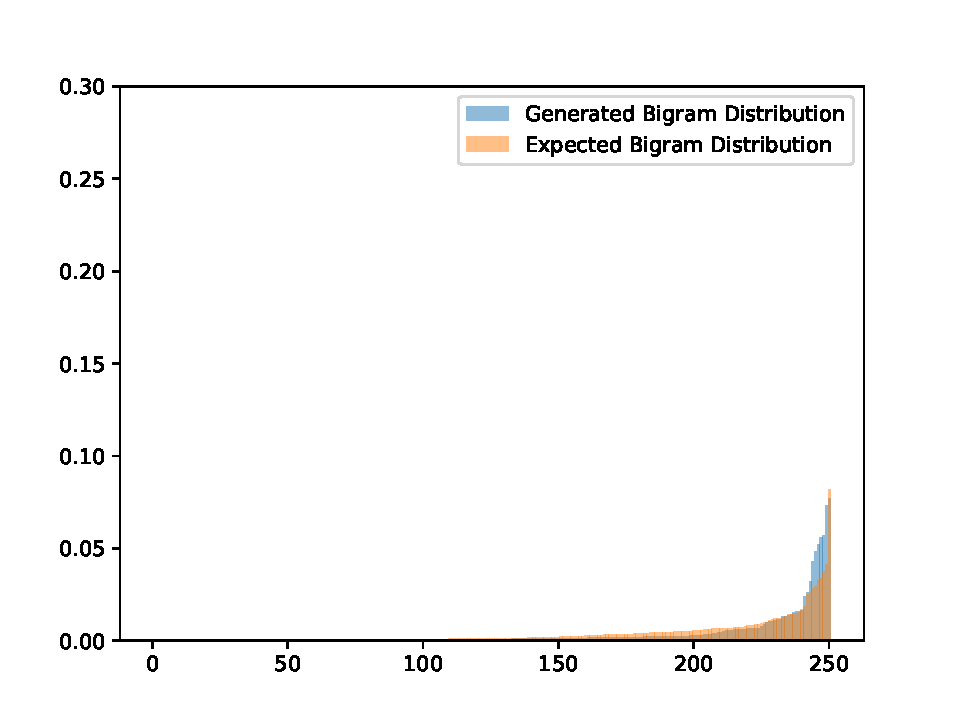
\includegraphics[width=\linewidth]{img/plots/reddit/bigram_distribution_comparison_step_1000000.pdf}
	\centering
	\small
	\text{Snapshot 1.0M}
	\endminipage\hfill
	\minipage{0.5\textwidth}
	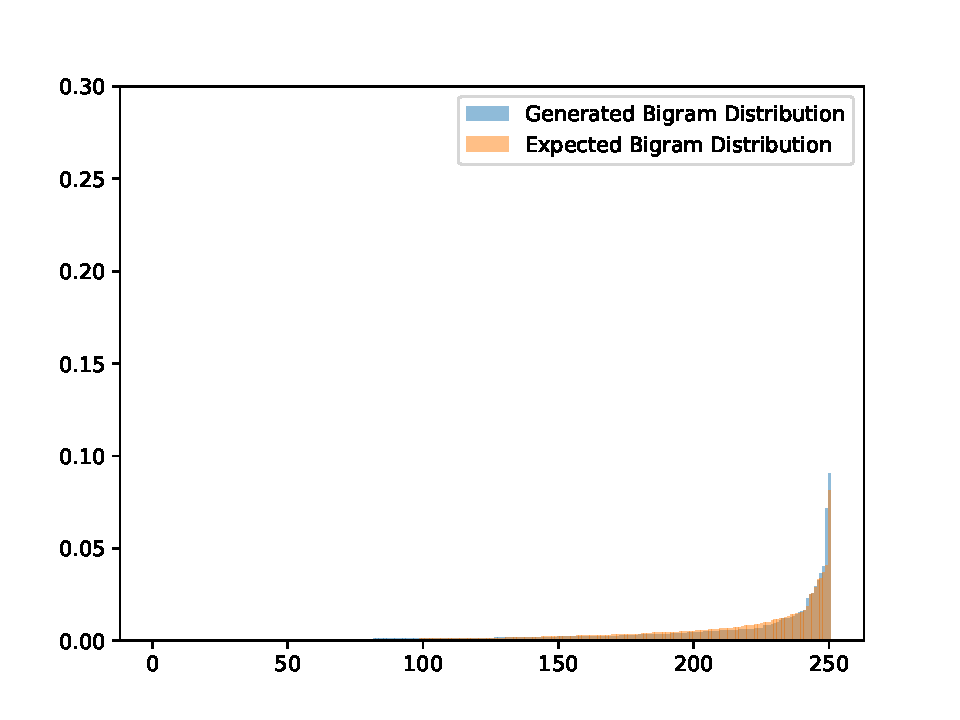
\includegraphics[width=\linewidth]{img/plots/reddit/bigram_distribution_comparison_step_1500000.pdf}
	\centering
	\small
	\text{Snapshot 1.5M}
	\endminipage\hfill
	\minipage{0.5\textwidth}
	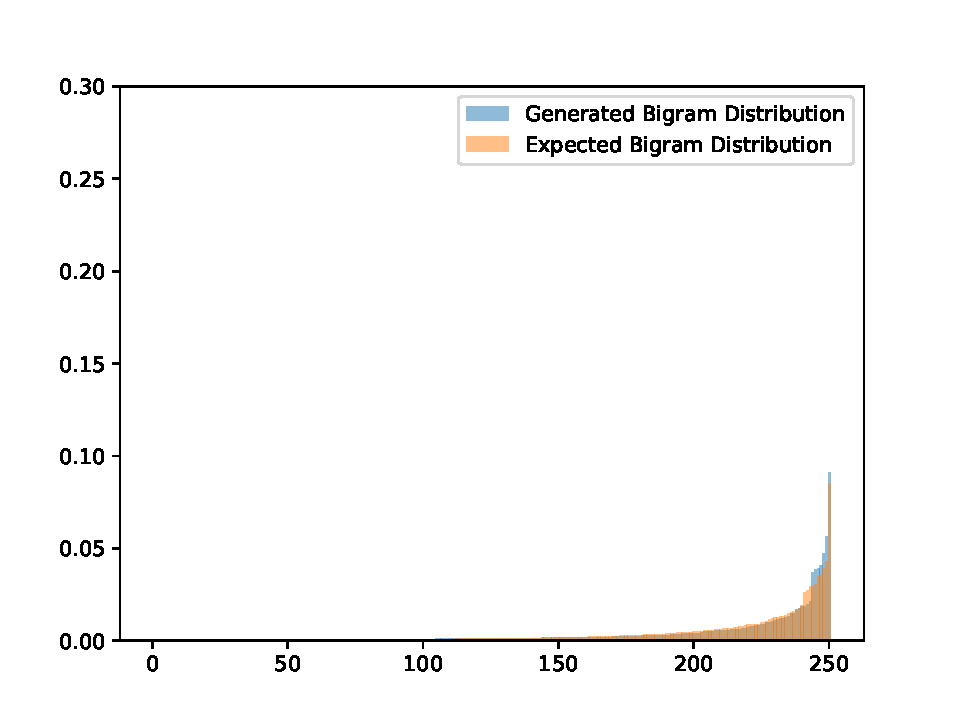
\includegraphics[width=\linewidth]{img/plots/reddit/bigram_distribution_comparison_step_2000000.pdf}
	\centering
	\small
	\text{Snapshot 2.0M}
	\endminipage\hfill
	\minipage{0.5\textwidth}
	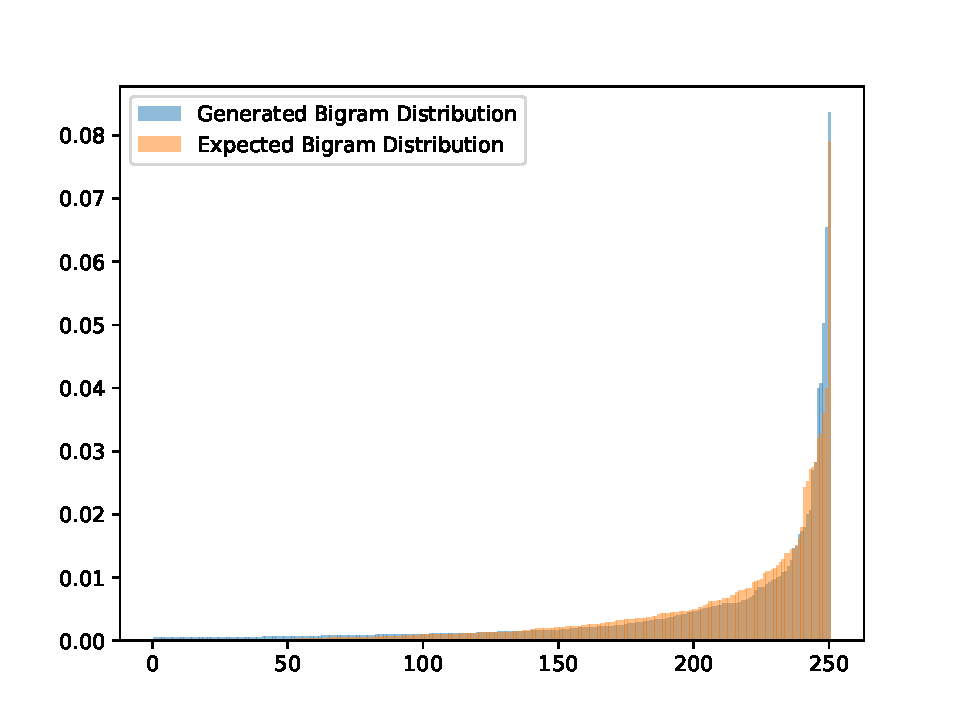
\includegraphics[width=\linewidth]{img/plots/reddit/bigram_distribution_comparison_step_2500000.pdf}
	\centering
	\small
	\text{Snapshot 2.5M}
	\endminipage\hfill
	\minipage{0.5\textwidth}
	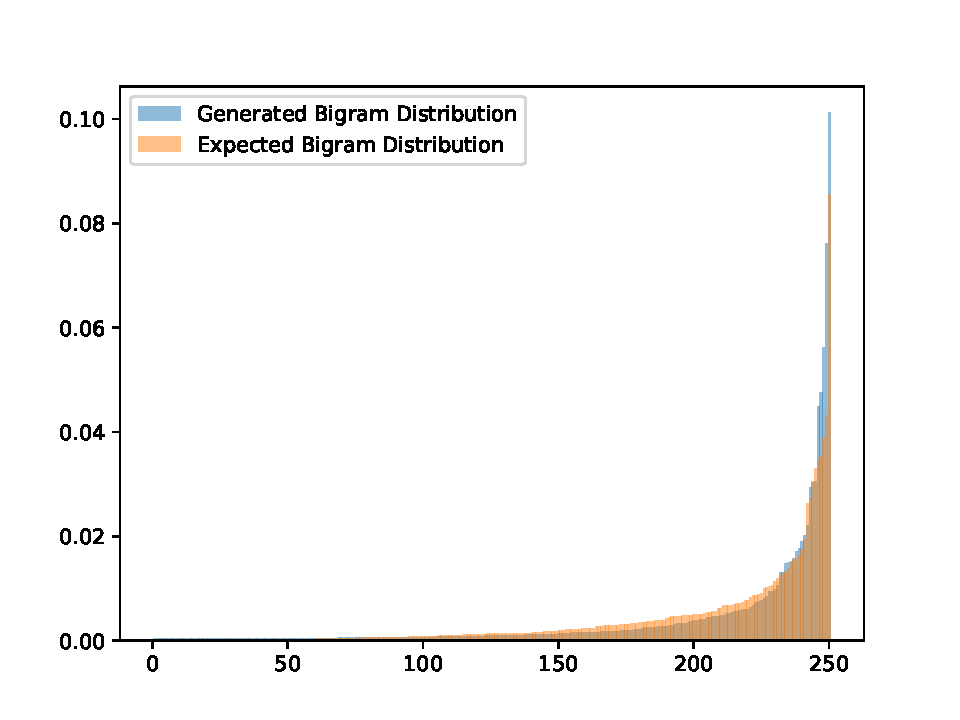
\includegraphics[width=\linewidth]{img/plots/reddit/bigram_distribution_comparison_step_3000000.pdf}
	\centering
	\small
	\text{Snapshot 3.0M}
	\endminipage\hfill
	\caption{Comparison of the distributions of the top 100 most used bigrams for the responses of the Reddit models (orange) when using the test dataset and the distribution within the training data (blue). The distributions are compared for each snapshot available.}
	\label{results:bigram:distributions:reddit}
\end{figure}

\begin{figure}[H]
	\minipage{0.5\textwidth}
	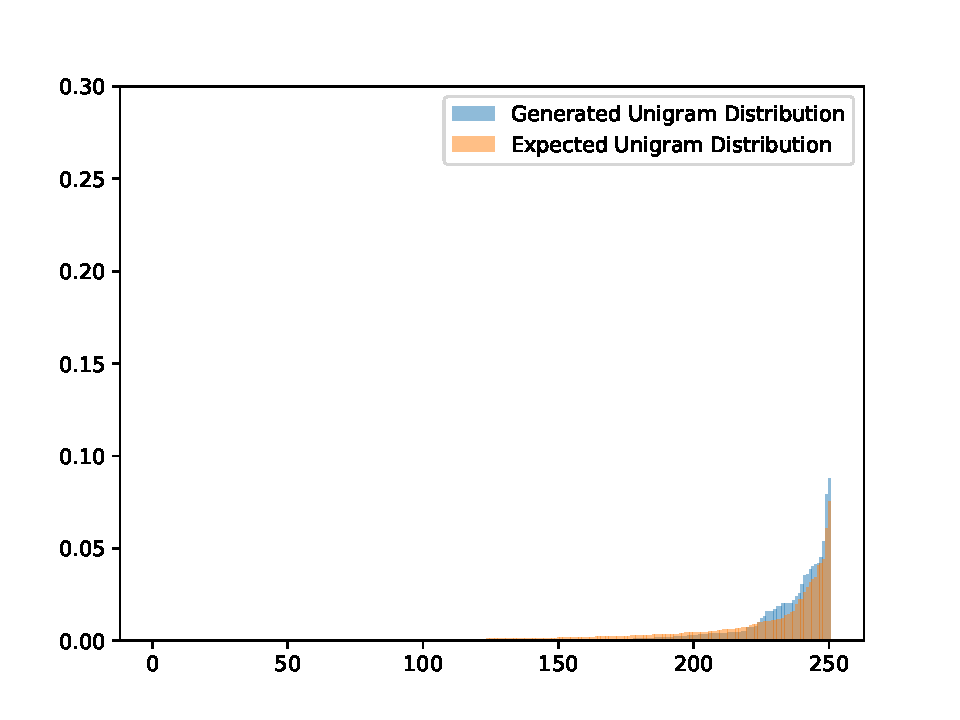
\includegraphics[width=\linewidth]{img/plots/opensubtitles_not_reversed/unigram_distribution_comparison_step_500000.pdf}
	\centering
	\small
	\text{Snapshot 0.5M}
	\endminipage\hfill
	\minipage{0.5\textwidth}
	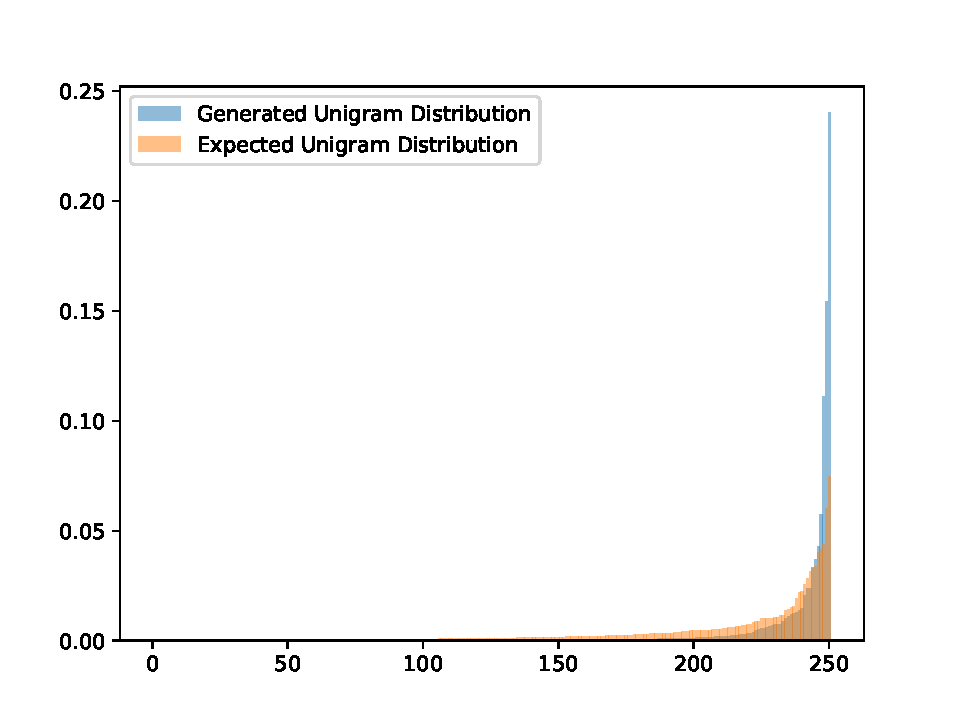
\includegraphics[width=\linewidth]{img/plots/opensubtitles_not_reversed/unigram_distribution_comparison_step_1000000.pdf}
	\centering
	\small
	\text{Snapshot 1.0M}
	\endminipage\hfill
	\minipage{0.5\textwidth}
	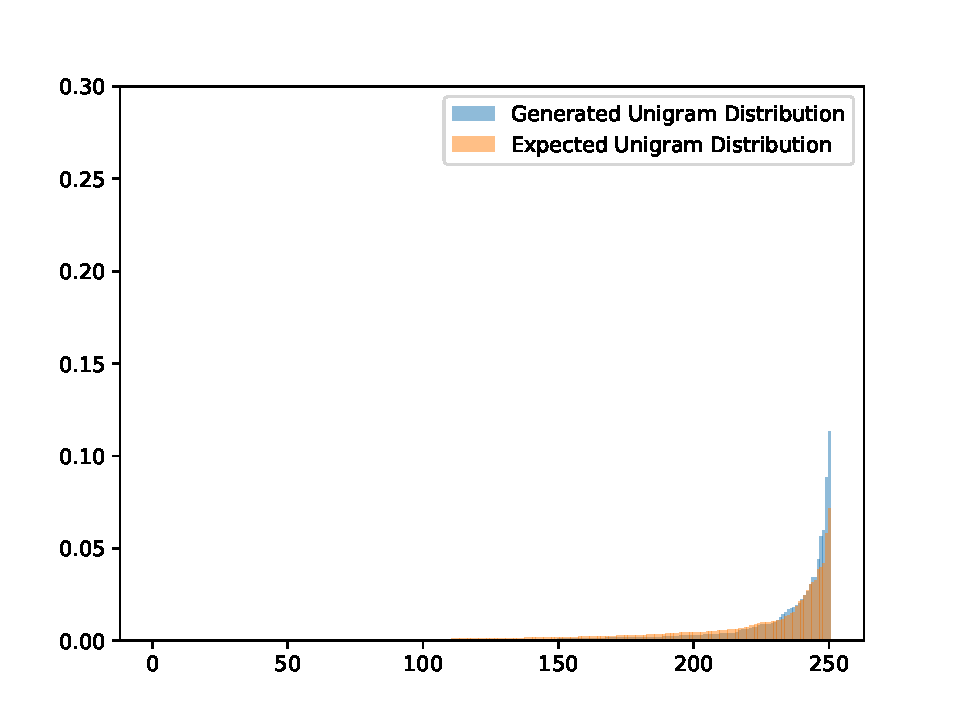
\includegraphics[width=\linewidth]{img/plots/opensubtitles_not_reversed/unigram_distribution_comparison_step_1500000.pdf}
	\centering
	\small
	\text{Snapshot 1.5M}
	\endminipage\hfill
	\minipage{0.5\textwidth}
	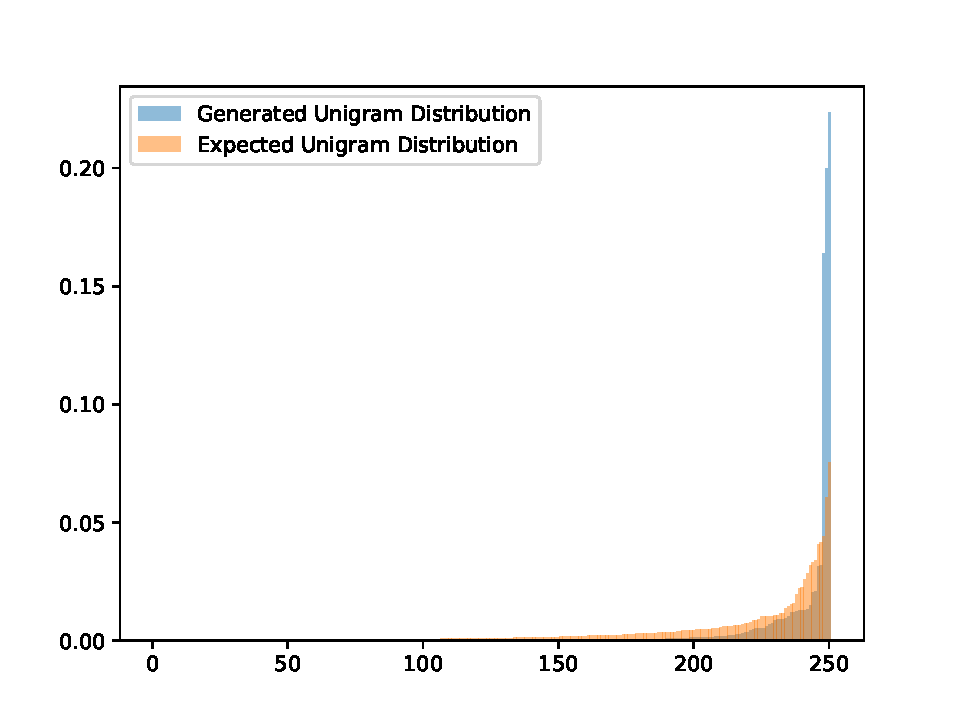
\includegraphics[width=\linewidth]{img/plots/opensubtitles_not_reversed/unigram_distribution_comparison_step_2000000.pdf}
	\centering
	\small
	\text{Snapshot 2.0M}
	\endminipage\hfill
	\minipage{0.5\textwidth}
	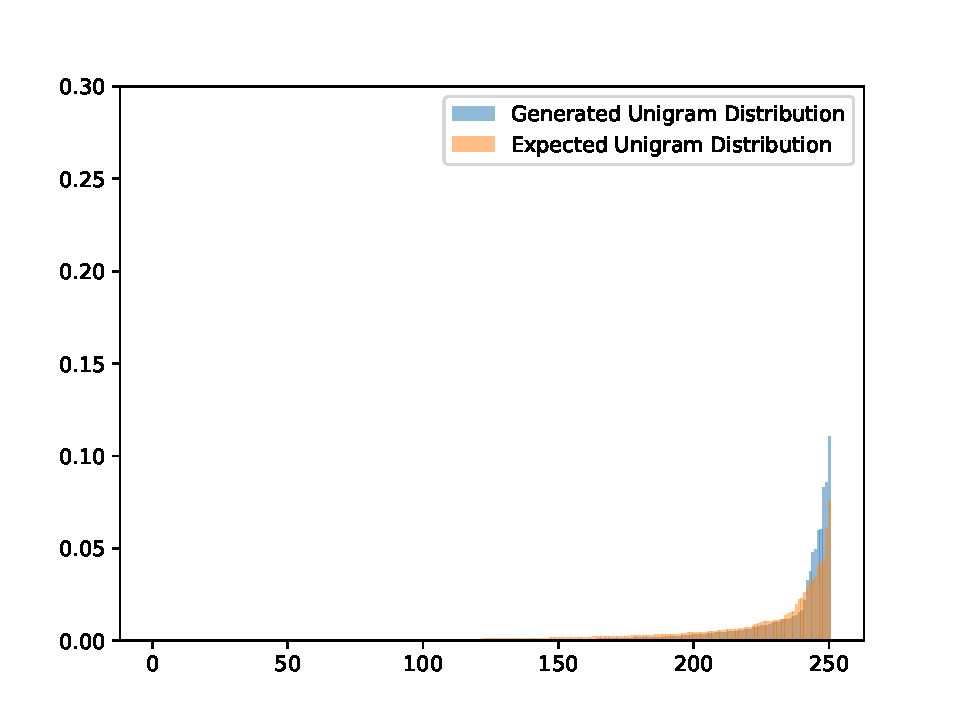
\includegraphics[width=\linewidth]{img/plots/opensubtitles_not_reversed/unigram_distribution_comparison_step_2500000.pdf}
	\centering
	\small
	\text{Snapshot 2.5M}
	\endminipage\hfill
	\minipage{0.5\textwidth}
	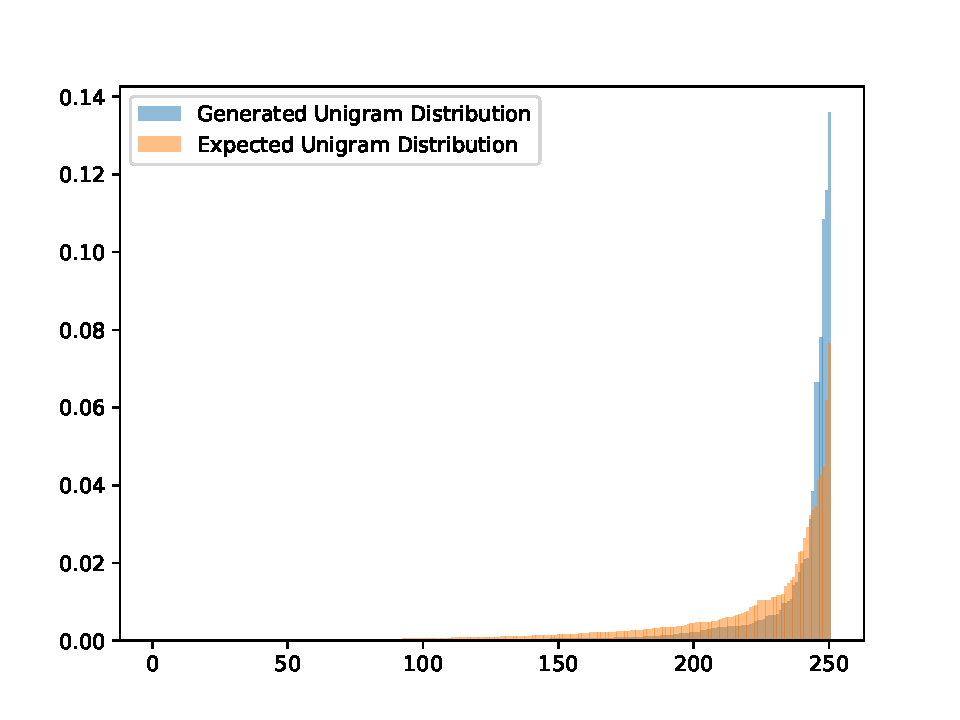
\includegraphics[width=\linewidth]{img/plots/opensubtitles_not_reversed/unigram_distribution_comparison_step_3000000.pdf}
	\centering
	\small
	\text{Snapshot 3.0M}
	\endminipage\hfill
	\caption{Comparison of the distributions of the top 100 most used unigrams for the responses of the OpenSubtitles models (orange) when using the test dataset and the distribution within the training data (blue). The distributions are compared for each snapshot available.}
	\label{results:unigram:distributions:opensubtitles}
\end{figure}

\begin{figure}[H]
	\minipage{0.5\textwidth}
	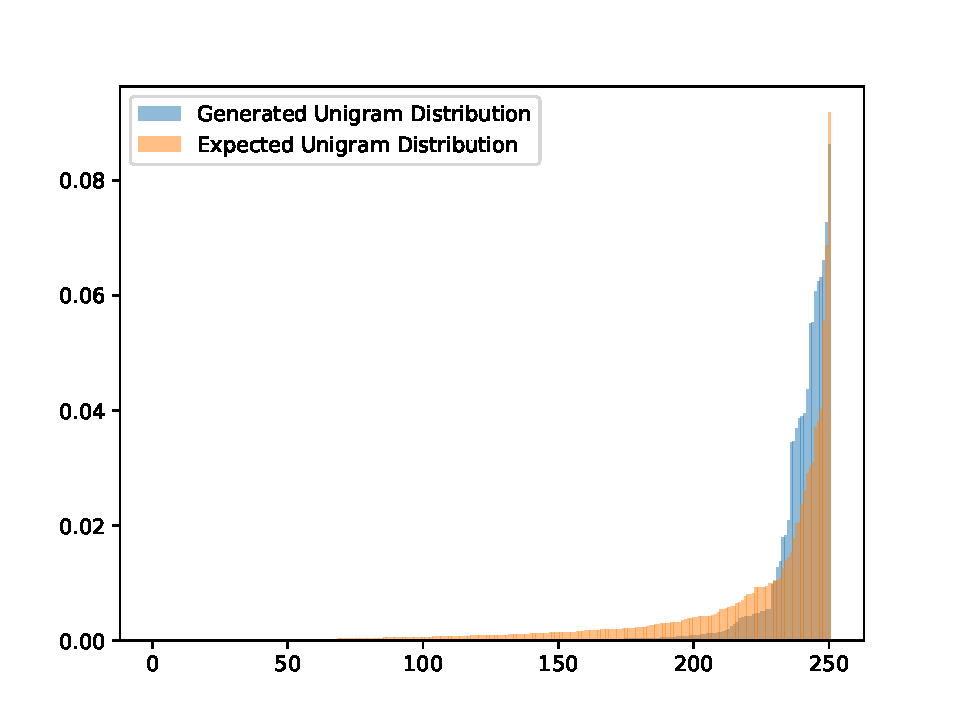
\includegraphics[width=\linewidth]{img/plots/reddit/unigram_distribution_comparison_step_500000.pdf}
	\centering
	\small
	\text{Snapshot 0.5M}
	\endminipage\hfill
	\minipage{0.5\textwidth}
	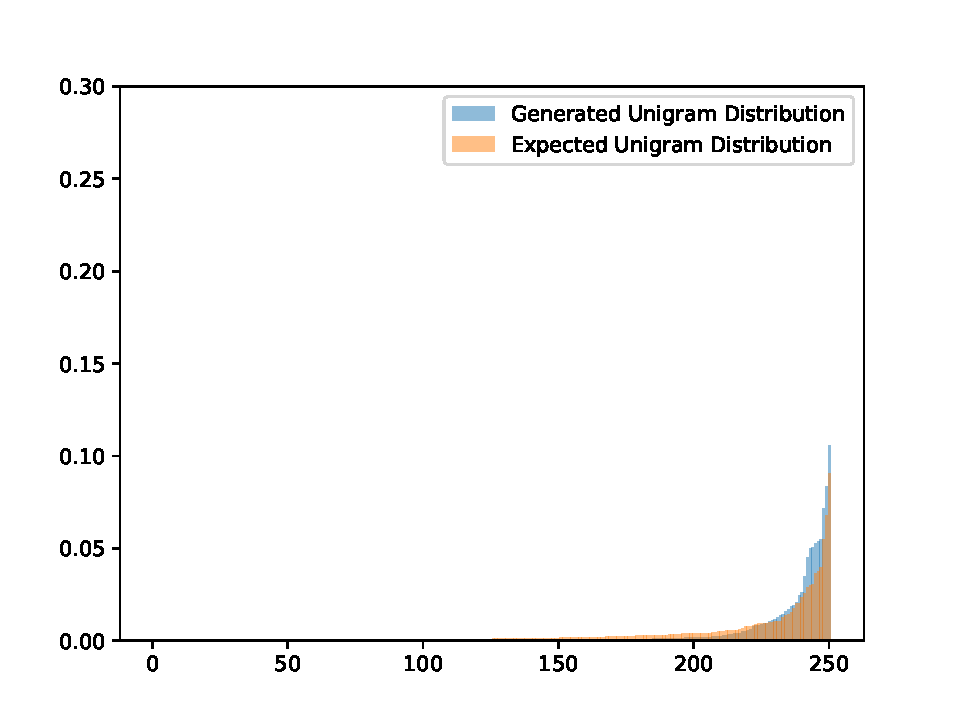
\includegraphics[width=\linewidth]{img/plots/reddit/unigram_distribution_comparison_step_1000000.pdf}
	\centering
	\small
	\text{Snapshot 1.0M}
	\endminipage\hfill
	\minipage{0.5\textwidth}
	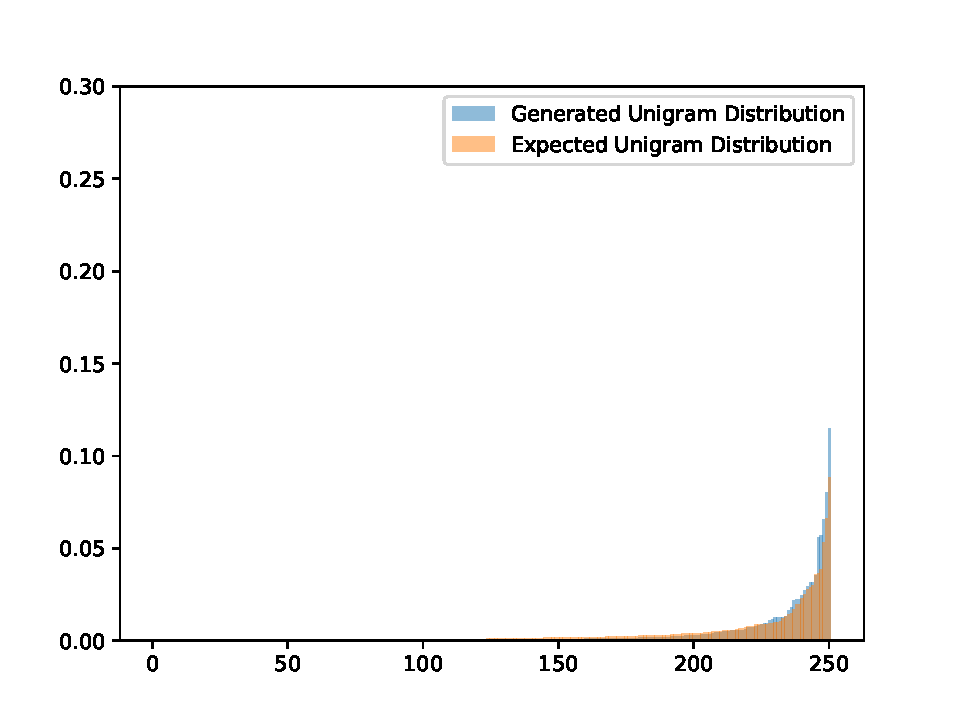
\includegraphics[width=\linewidth]{img/plots/reddit/unigram_distribution_comparison_step_1500000.pdf}
	\centering
	\small
	\text{Snapshot 1.5M}
	\endminipage\hfill
	\minipage{0.5\textwidth}
	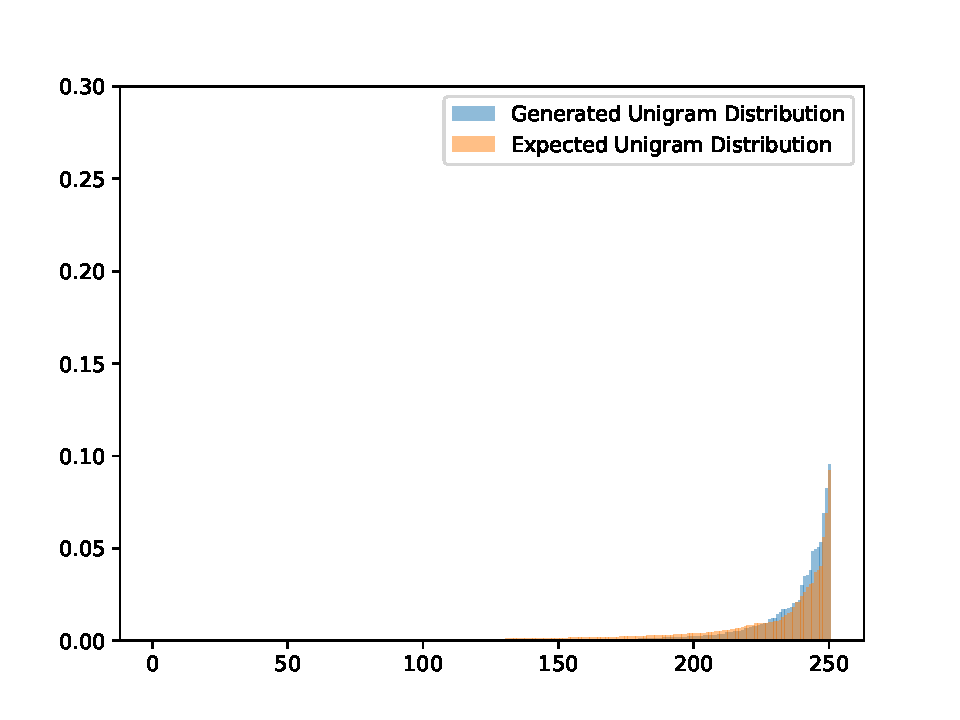
\includegraphics[width=\linewidth]{img/plots/reddit/unigram_distribution_comparison_step_2000000.pdf}
	\centering
	\small
	\text{Snapshot 2.0M}
	\endminipage\hfill
	\minipage{0.5\textwidth}
	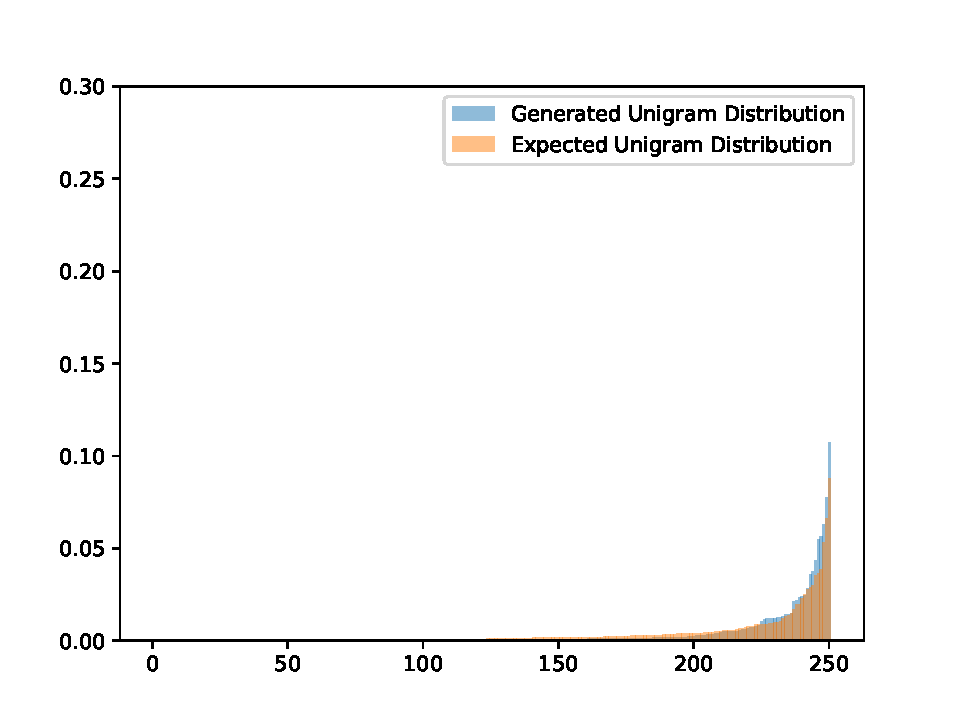
\includegraphics[width=\linewidth]{img/plots/reddit/unigram_distribution_comparison_step_2500000.pdf}
	\centering
	\small
	\text{Snapshot 2.5M}
	\endminipage\hfill
	\minipage{0.5\textwidth}
	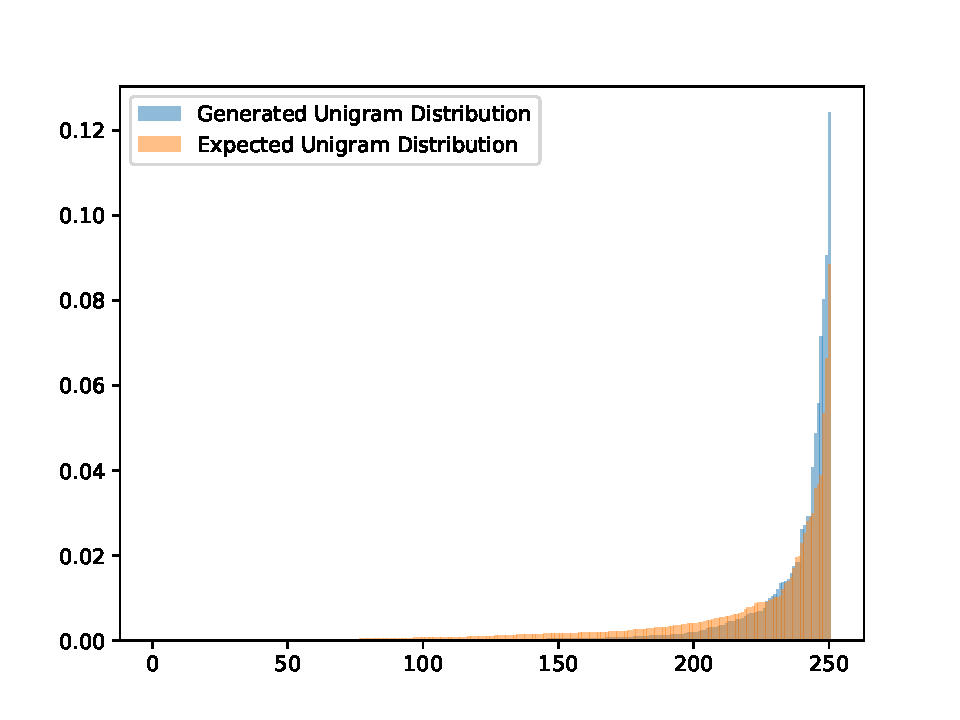
\includegraphics[width=\linewidth]{img/plots/reddit/unigram_distribution_comparison_step_3000000.pdf}
	\centering
	\small
	\text{Snapshot 3.0M}
	\endminipage\hfill
	\caption{Comparison of the distributions of the top 100 most used unigrams for the responses of the Reddit models (orange) when using the test dataset and the distribution within the training data (blue). The distributions are compared for each snapshot available.}
	\label{results:unigram:distributions:reddit}
\end{figure}

\subsection{Bi-Gramm}
In den Grafiken \ref{results:ngram:distributions:opensubtitles} und \ref{results:ngram:distributions:reddit} wird dargestellt (erklären, was genau man sieht, muss genau sein, da nicht ganz einfach.)
\paragraph{Die bi-gramme und deren Wahrscheinlichkeiten werden übernommen.}
\todo{grafiken interpretieren}
\paragraph{The distribution is right-handed} of the words... Für beide Modelle gilt: Starten gleichverteilter, als expected, nähern sich dann dem expected Werten an. Dieser Virgang scheint von links nacht rechts stattzufinden. Das scheint insofern nachvollziehbar, dass er schnell merkt, welche bi-gramme nicht oft vorkommen und entsprechend diese fast nie verwendet.Jedoch herauszufinden, welches der top n n-gramme das Richtige ist, ist ein deutlich schwierigerer Lernprozess. Wir sehen im groben zumindest eine Annäherung der Verteilung. Wünschenswert wäre natürlich hier eine ähnliche Verteilung wie expected, wobei vor allem die weniger häufigen Bigramme für eine vielfältige Sprache stehen. Dies würde sich ganz generell als mass für die Sprachvielfalt eigenen, indem man z.B. die umgekehrte Wahrscheinlichkeit als Gewicht Einfliessen lässt.

\subsection{Uni-gramm/Wörter}
\todo{grafiken erstellen und referenzieren und beschreiben}
\paragraph{Die Uni-gramm und deren Wahrscheinlichkeiten werden übernommen.}
\todo{grafiken interpretieren}
\paragraph{The distribution is}
\todo{grafiken interpretieren}

\subsection{Does the Model have an understanding of natural language sentiment?}

\paragraph{Thought Vectors for Input Sequences}After the encoder has processed the whole input sequences, it pass it forward to the decoder to construct the output sequence (see Chapter~\ref{fundamentals:seq2seq}). It is the only direct connection the encoder and decoder have in such a model, which means, that the encoder has to ``encode'' all the information into this thought vector before passing it to the decoder. The thought vector hence represents an embedding of the input sequence in an $n$ dimensional vector space, where $n$ stands for the size of the thought vector. To analyze this embeddings, we collected them for 15 different sample sentences and projected them via PCA into two dimensional space, the results of this projection can be see in Figure~\ref{results:thougth_vectors:embeddings:opensubtitles} and~\ref{results:thougth_vectors:embeddings:reddit} below.

\begin{figure}[H]
	\centering
	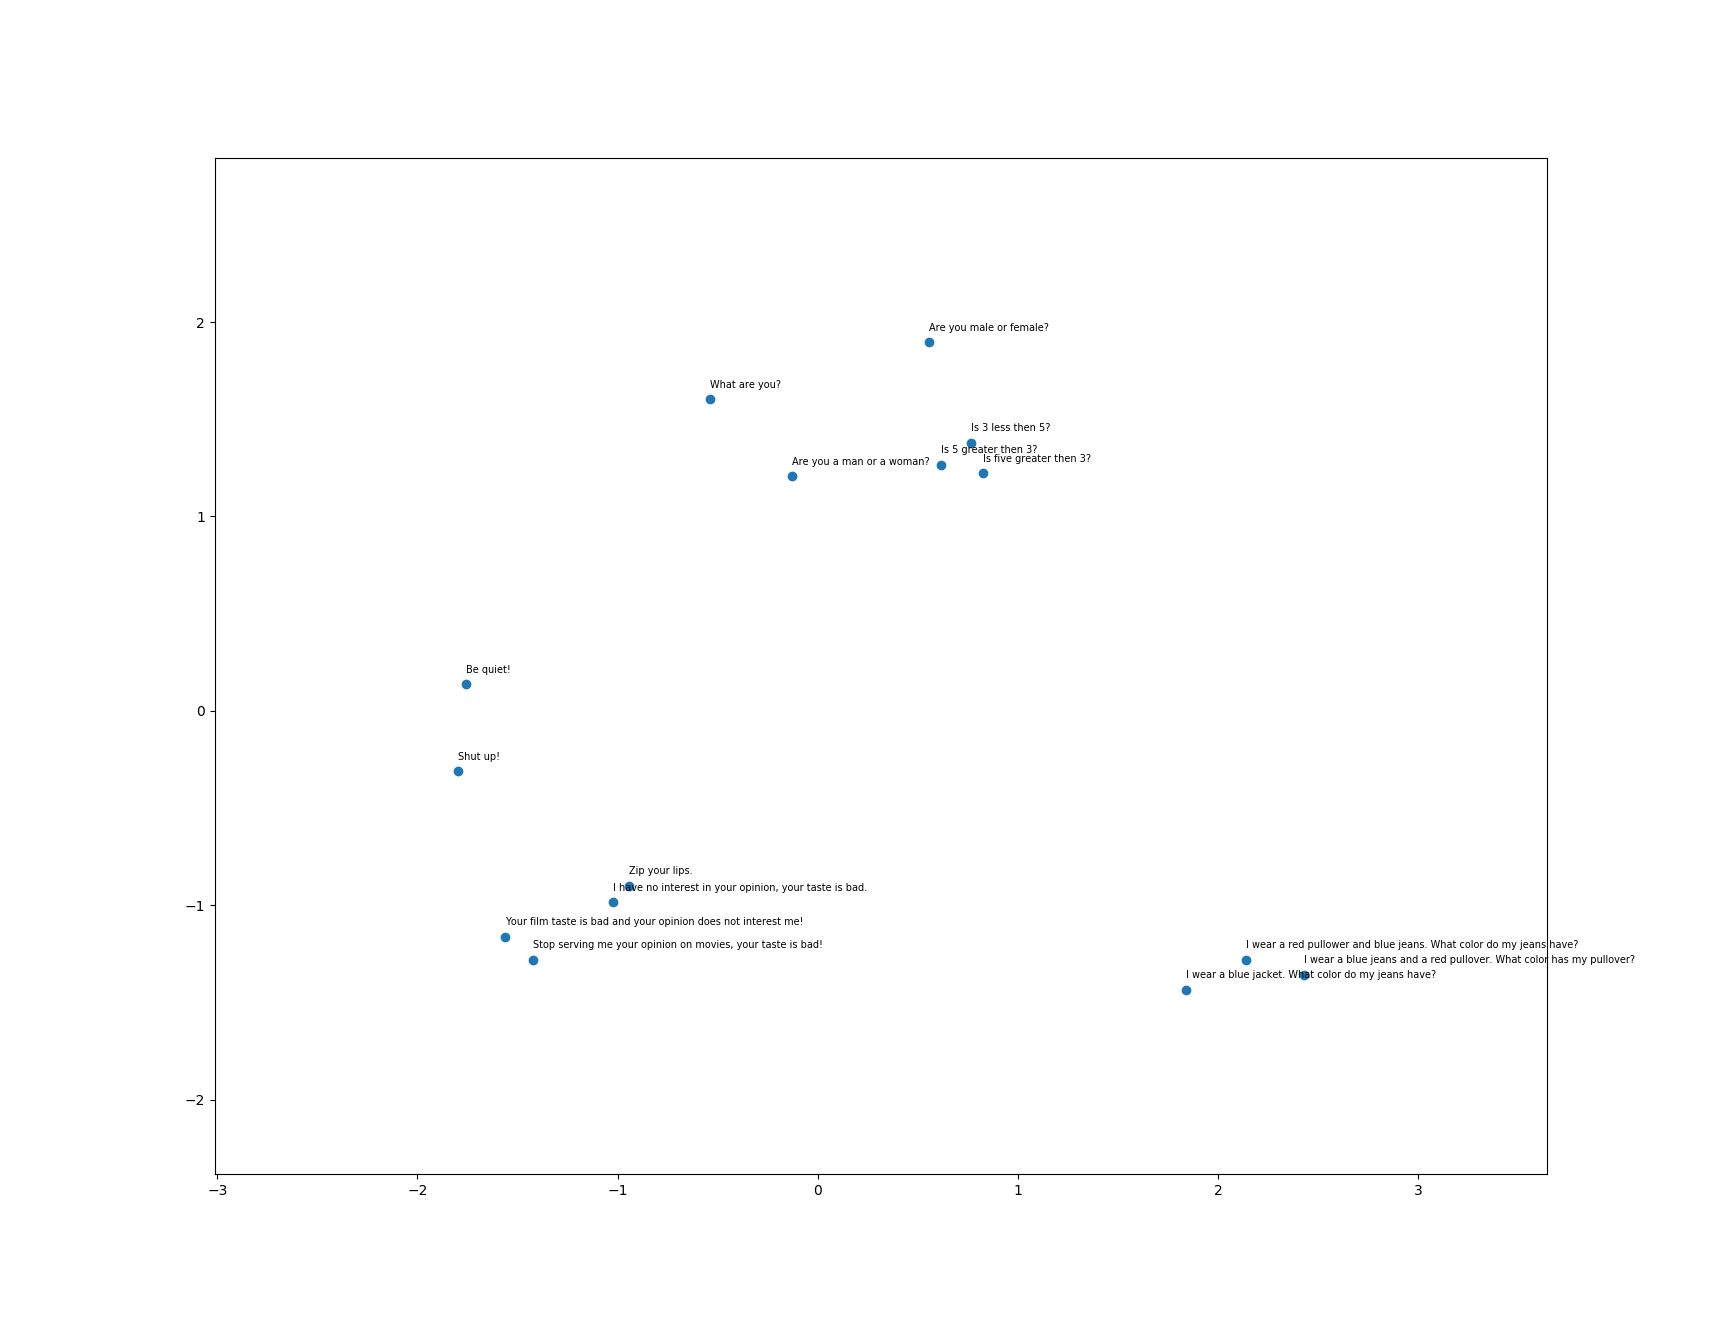
\includegraphics[width=16cm]{img/opensubtitles_thought_vector_embeddings.png}
	\caption{The projected thought vectors for 15 different sentences when using the OpenSubtitles model. PCA was used for the projection.}
	\label{results:thougth_vectors:embeddings:opensubtitles}
\end{figure}

\begin{figure}[H]
	\centering
	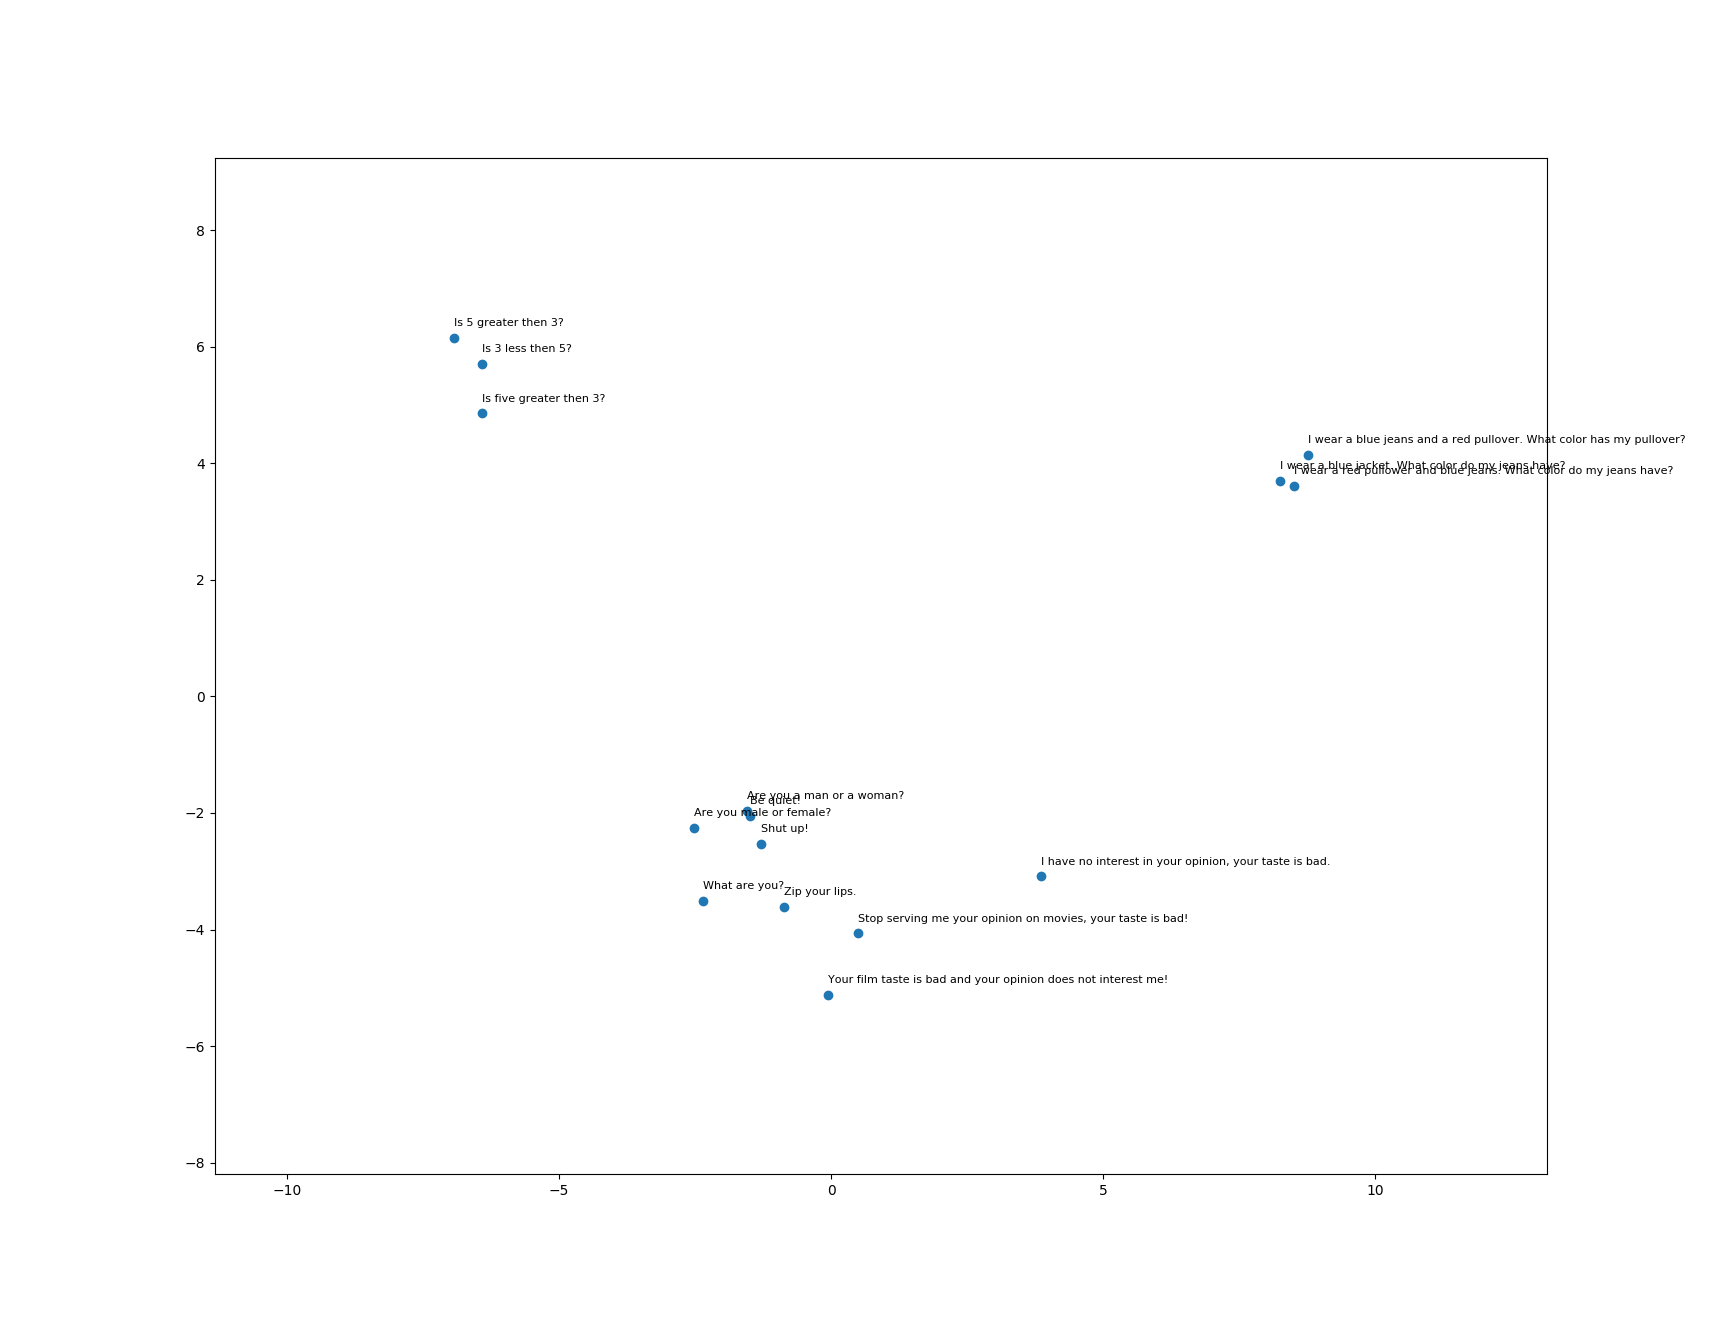
\includegraphics[width=16cm]{img/reddit_thought_vector_embeddings.png}
	\caption{The projected thought vectors for 15 different sentences when using the Reddit model. PCA was used for the projection.}
	\label{results:thougth_vectors:embeddings:reddit}
\end{figure}

Both of the models seem to have no problems understanding clear, direct sentences where the intent is clear (e.g. ``I have no interest in your opinion on movies, your taste is bad!''). This can be seen because similar sentences are clustered together in the projected space. However, when it comes to curses and questions regarding the gender, the OpenSubtitles model starts to struggle, which can be seen by taking a look at the respective points in the projected space. For example, the questions regarding the gender or the curses are scattered throughout the space, even though they should have been embedded closely to each other. The Reddit model seems to have less problems with this, as the embeddings for these sentences are quite close together. But what is interesting to see is that the Reddit model embeds the sentences with curses close to the sentences regarding the gender.\todo{write more}



\section{What Language Model do the Models produce?}
\blindtext

\section{Does the Model have an understanding of natural language?}
\blindtext

\section{How can we fix the detected problems?}
\blindtext



\section{Generated outputs over time}
\blindtext

\section{Comparison with CleverBot and ``Neural Conversational Model''}
\blindtext


\section{Reverse Input Feeding}
\blindtext